%!TEX root = ../template.tex
%%%%%%%%%%%%%%%%%%%%%%%%%%%%%%%%%%%%%%%%%%%%%%%%%%%%%%%%%%%%%%%%%%%
%% vanet.tex
%% NOVA thesis document file
%%
%% Chapter with introduction
%%%%%%%%%%%%%%%%%%%%%%%%%%%%%%%%%%%%%%%%%%%%%%%%%%%%%%%%%%%%%%%%%%%

\typeout{NT FILE vanet.tex}%

\chapter[Vehicular Ad hoc Networks]{\glsxtrlongpl{vanet}} % (fold)
\label{cha:vehicular_networks}

% Introduction to vehicular ad hoc network
% Motivation to bring connectivity to moving vehicles
The automobile was one of the most revolutionary inventions in human history, for most cities around the world are dependent on cars for the transportation of goods and people and, therefore, the prevalence of vehicles in our daily lives is greater than ever before. Even though it is impossible to predict if future vehicle usage will continue to be as dominant as today, it is reasonable to assume that this technology will never disappear completely. Even today, in cities dominated by alternative modes of transportation, the use of motorized vehicles is still present and, in some cases, a necessity.

It has been a long-time goal for car manufacturers and researchers to bring internet connectivity to automobiles, as the benefits are enormous. The Internet is an extremely powerful technology, not only for the countless services it provides but also for the ability of two endpoints to communicate almost instantly. Moreover, recent improvements to wireless communication technologies not only make this goal more realistic but also even more attractive, as integrating network interfaces with \gls{gps} receivers and sensors only increases the potential of allowing cars to communicate with each other~\cite{jakubiak_state_2008}.

% Definition of vehicular ad hoc networks
The efforts to bring connectivity to automobiles resulted in the emergence of the technology named \gls{vanet}, which is an adaptation of the \gls{manet} technology, specialized for automobiles~\cite{al-sultan_comprehensive_2014}~\cite{liang_vehicular_2015}. In contrast to wired networks, where all devices are connected to the infrastructure at all times to communicate with each other, this technology allows devices to transmit data directly to other devices inside its range, as illustrated in Figure~\ref{fig:ad_hoc}. As a result, networks are generated spontaneously between nodes that are in range of each other, which makes topologies unstable and requires each node in the network to act as both a transmitter and a receiver. 

\begin{figure}[htbp]
	\centering
	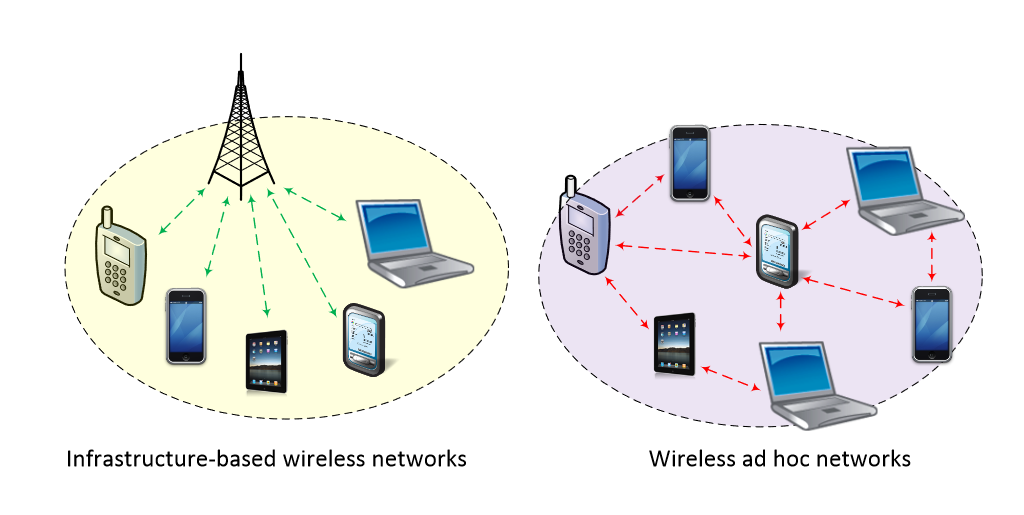
\includegraphics[width=0.8\textwidth]{Chapters/Figures/VANETs/ad_hoc_networks.png}
	\caption{Comparison between infrastructure networks~\cite{dinh_thai_applications_2015}}
	\label{fig:ad_hoc}
\end{figure}

% Architecture of VANET

As the Internet was not designed with mobility in mind, most protocols and standards were not developed to support the high-speed scenarios of \gls{vanet}. A tremendous amount of work and research efforts has already been conducted in this area, amounting to decades of research, development, and standardization. However, the development of \gls{vanet} technology began without any major centralized entity to standardize its implementation worldwide, resulting in various architectures emerging simultaneously all around the globe. It is common for different regions of the world to develop different standards for infrastructure-related technologies and these solutions tend to converge as they seek to solve the same problems in the most optimal way. 

The leaders in global research on \glspl{vanet} are considered to be the \gls{us}, Japan, and the \gls{eu}. These regions are noteworthy as they have provided the majority of the technological foundations and advancements in the field. For the sake of clarity and relevance, this document focuses on the European \glspl{vanet} architecture through the discussion of the \gls{c2c} and the \gls{etsi}, two prominent and influential institutions in the field. 

The \gls{c2c} architecture proposal is designed with a high level of abstraction and is therefore fairly easy to understand. In contrast, the \gls{etsi} standards are significantly more detailed and technical, since they provide the official standard for the \gls{eu}. \gls{etsi} uses the term \gls{its} to refer to \glspl{vanet}, as their efforts to connect vehicles together goes beyond cars and aims to interconnect planes, trains, boats, etc.

There are other conventions in this field, such as the C-ROADS platform~\cite{noauthor_platform_nodate}, which are important for the development of this technology. In fact, several conventions have influenced the \gls{etsi} standards and would be worth discussing. However, in order to avoid overcomplicating the subject, only the \gls{etsi} and \gls{c2c} architectures will be covered.

% Explain what the sections talks about
%This section begins by delving into the peculiarities of \glspl{vanet}, followed by a review of the main components and domains of this technology. This chapter continues by examining \glspl{vanet} with a communication-oriented vision right before exploring all layer and component in the \glspl{etsi} standardized architecture. Then, \gls{vanet} simulation tools will be explored, concluding with some notes on the future of this technology.



\section[VANET characteristics]{\gls{vanet} characteristics}
\label{sec:VANET_characteristics}

% Introduction
The \gls{vanet} technological domain was established as a specialized subset of the \gls{manet} research field based on some unique characteristics, and thus \gls{vanet} shares most of its properties with \gls{manet}. Some key differences require the development of novel solutions, and in this section, we will go through all the characteristics of \gls{vanet} while shedding light on what sets this technology apart from its origin.

    % Characteristics
        % High mobility 
\subsection{High mobility}
\label{subsec:high_mob}

\gls{manet} topologies are highly dynamic, driven by the mobility of nodes. High mobility leads to uncertain connectivity, which makes ad-hoc topologies extremely volatile and unpredictable, with a high chance of partitions~\cite{toor_vehicle_2008}. \glspl{vanet} not only inherit this characteristic but also amplify its volatility since \gls{vanet} nodes are vehicles capable of traveling at extremely high speeds. 

For instance, two cars traveling in opposite directions on the same road will only be within range of each other for a few seconds. In this short time, the vehicles must attempt to establish a connection before attempting to exchange valuable information, which means some links may be disconnected before there is a chance to use them~\cite{liang_vehicular_2015}. On the other hand, two cars traveling in the same direction can maintain a connection indefinitely as long as they keep on the same path at the same speed. These two scenarios are polar opposites, making the reliability of connections inconsistent.

% Predictable mobility
\subsection{Predicted mobility}
\label{subsec:predicted_mob}

Beyond being more dynamic, \gls{manet} topologies are also random, as nodes can move arbitrarily and at unpredictable times, with virtually no restraint. \gls{vanet} topologies diverge from \gls{manet} in this matter, as it is possible to reliably predict the path of nodes in an ad-hoc network. Vehicles are primarily used on pre-built infrastructure~\cite{liang_vehicular_2015}, like roads and motorways, and have to follow predetermined paths to reach their destination, which makes it possible to predict their future location. Vehicles are also forced to obey road signs and traffic lights and have to respond to other vehicles' movements~\cite{al-sultan_comprehensive_2014}, making topologies even more predictable.

On top of all of that, if drivers disclose their desired destination it becomes possible to predict the complete route of a node with near 100\% precision. It is important, however, to keep in mind that this is not always true, and in some instances, drivers may adjust their path in reaction to the information received by the network~\cite{liang_vehicular_2015}.

A negative consequence of road use can be seen in more linear topologies when compared with \glspl{manet}, which inevitably undermines path redundancy~\cite{toor_vehicle_2008}.

% High computational ability and no power constraints:
\subsection{Power and Computational ability}
\label{subsec:power_compute}

Another relevant change from \glspl{manet} is the computational capabilities and power constraints of the nodes. \gls{manet} was designed with small devices in mind, which have limited battery capacity and computational power constraints. In contrast, vehicles have access to a reliable power source~\cite{liang_vehicular_2015}~\cite{jakubiak_state_2008}, so there are essentially no concerns in this regard. However, cars should not be thought of as an infinite power source, and normal precautions should be taken when optimizing routing algorithms, etc.

% Congestion and scalability issues
\subsection{Congestion and Scalability issues}
\label{subsec:congestion_scalability}

\gls{vanet} suffers from an absurdly variable node density. A vehicle can be on a road in a remote location with the nearest internet connection of other vehicle kilometers away from their location, or in the middle of a traffic jam at an intersection surrounded by hundreds of vehicles all trying to communicate within its range.

Congestion scenarios create a bandwidth problem that is exacerbated by the presence of nearby obstacles like other cars and buildings, which common in an urban environment~\cite{toor_vehicle_2008}. Wireless links are significantly more fragile than their wired counterparts because they are subject to fading, noise and interference~\cite{corson_mobile_1999}. This also forces researchers to come up with effective measures for sharing physical media, as another issue of concern is ensuring \gls{qos} measures for critical messages, like road hazard warnings, which presents a core issue~\cite{toor_vehicle_2008}.
 
Variable network density presents a necessity for the protocols developed to be capable of dealing with any situation thrown at them in the real world.


\section[VANET components]{\gls{vanet} components}
\label{sec:VANET_components}

% Typical components
The first step in the understanding \gls{vanet} scenarios is the analysis of the basic elements involved. With this in mind, the atomic components of both the \gls{c2c} and \gls{etsi} are explained in this section.

\subsection[C2C approach]{\gls{c2c} approach}
    % C2C-CC
According to the \gls{c2c} architecture, three main components can be identified, these being the \gls{rsu}, \gls{obu} and \gls{au}.

\begin{enumerate}
        	% Roadside Units (RSUs)
	\item \glsxtrlongpl{rsu} are stationary devices placed alongside roads, usually in high-density zones such as junctions, intersections and traffic lights.

    These devices have a reliable connection to the Internet and communicate with all vehicles within their effective range, bridging the gap between vehicle ad hoc networks and the rest of the Internet. \glspl{rsu} can also be equipped with multiple communication devices for optimal wireless connectivity. In addition, \glspl{rsu} can also take advantage of the ad hoc characteristics of on-board units by using them as transmitters, thereby extending their effective range, as depicted on Figure~\ref{fig:RSU_range}.

    \begin{figure}[htbp]
    	\centering
    	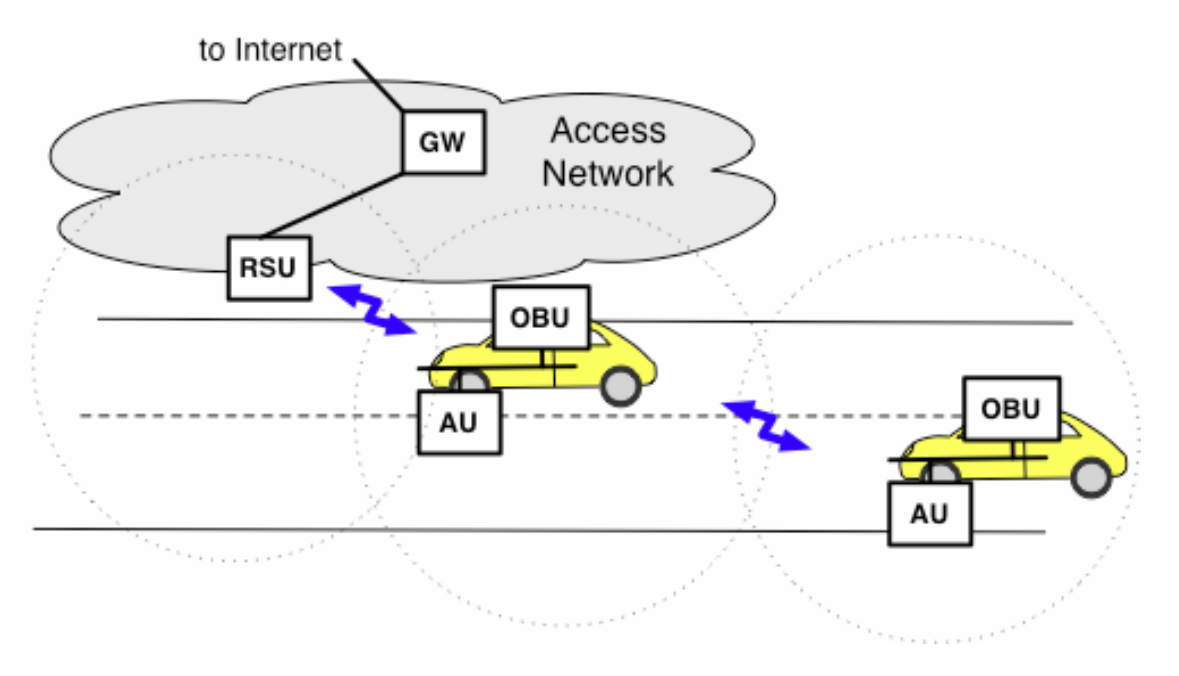
\includegraphics[width=0.8\textwidth]{Chapters/Figures/VANETs/c2c-cc_RSU_range.png}
    	\caption{A \gls{rsu} provides Internet connectivity through an \gls{obu}.~\cite{c2c-cc_car_2007}}
    	\label{fig:RSU_range}
    \end{figure}

    \glspl{rsu} can run safety applications like fixed road hazard warnings (work-zone warnings, bridge warnings, etc.) by broadcasting safety messages to nearby vehicles, making them more than mere connection points for vehicles.
    
        	% On-Board Units (OBUs)
	\item \glsxtrlong{obu} is a small device integrated into vehicles that operates in the ad hoc space as they receive, send, and forward messages between each other and with \glspl{rsu} in an ad hoc manner. \glspl{obu} provide it's wireless communication capabilities to any connected device used within the vehicle.
 
        	% Autonomous Units (AUs)
	\item The term \glsxtrlongpl{au} refers to all the various devices that run a single or a set of applications that connect to the \gls{obu} and harness its wireless capabilities. The \glspl{au} can be physically integrated or permanently wired to the \gls{obu} being an integrated part of the vehicle. These types of \glspl{au} are typically safety-related applications. \glspl{au} can also be wireless devices like laptops or smartphones, wirelessly connecting to an \gls{obu} and utilizing its capabilities for leisure applications.

    % Others
    \item In addition to these three main components, this institution acknowledges the potential presence of other network entities, like public hotspots, instances of a Mobile \gls{ip} infrastructure, application servers, control centers, etc. However, these are not categorized and are therefore outside of the scope of this Consortium.

\end{enumerate}

\subsection[ETSI approach]{\gls{etsi} approach}
%ETSI

The \gls{etsi} standard diverges from the simple and straightforward definition of the \gls{c2c} by specifying two categories to define the communication entities of \glspl{vanet}: the \gls{its} sub-systems and the functional components. The former, comparable to the \gls{c2c} components, represent similar system categories that exist in the \gls{vanet} space. The latter are the building blocks that make up the \gls{its} sub-systems and are therefore responsible for specific functions or tasks within the overall systems.

\subsubsection{Functional components}
% Functional components

The functional components described in this architecture follow the layered conceptual structure of the \gls{osi} model~\cite{etsi_intelligent_2010}, comprising five such components: the \gls{its-s} host, the \gls{its-s} gateway, the \gls{its-s} router, the \gls{its-s} border router and the \gls{its-s} interceptor.

The most significant component of this architecture is the \gls{its-s} host, since it provides the minimum level of functionality required to run \gls{its} applications. It represents the basic reference architecture for any device wishing to communicate in the \gls{vanet} space, and is present on all \gls{its} sub-systems. This architecture is described in depth in section \ref{sec:vanet_arch} 

In addition, all other components are a variant of the \gls{its-s} host, adding communication capabilities to it. The \gls{its-s} gateway converts messages from the Internet to the \gls{its} domain at layers 5 to 7 of the \gls{osi} model. The \gls{its-s} router converts various \gls{its} protocols at layer 3, and the \gls{its-s} border router performs a similar task, doing the same as the router, but with a more generic network, without management or security awareness. The \gls{its-s} interceptor is a generic term equivalent to any of the previous three components, plus it can represent an implementation-specific connection of the \gls{its} station-internal network to another network.

\subsubsection{Sub-systems}
%Sub-systems

As previously introduced, all functional components come together to form various sub-systems, of which there are four. These sub-systems represent a specific context in which the functional components combine to attempt to provide wireless communication capabilities, either in the form of direct contact with the ad hoc environment or indirectly.

All \gls{its} sub-systems consist of the unique context they support and a specific \gls{its} station to meet the needs of that unique situation. These stations can also be implemented in a single physical unit or in multiple physical units.


\begin{enumerate}
        	% Personal 
	\item Personal \gls{its} sub-system:

The Personal \gls{its} sub-system represents a mobile or other personal device that can connect to the vehicle's internal network and use its ad-hoc wireless capabilities. It includes the user's device and a Personal \gls{its} Station. This station is the simplest of the four, consisting of a single \gls{its} host. This can be observed in Figure \ref{fig:personal_its}.

\begin{figure}[htbp]
    \centering
   	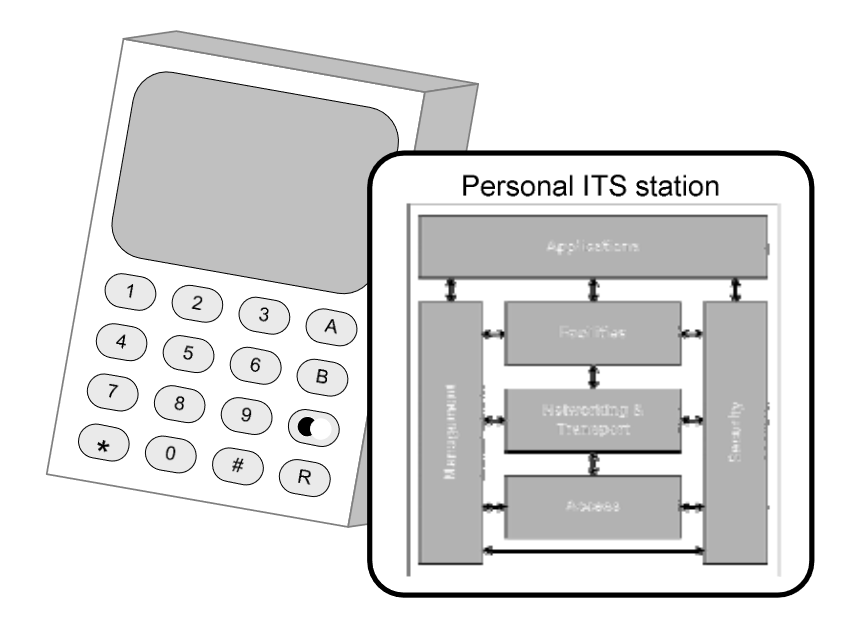
\includegraphics[width=0.8\textwidth]{Chapters/Figures/VANETs/personal_ITS.png}
   	\caption{Personal \gls{its} station in a Personal \gls{its} sub-system~\cite{etsi_intelligent_2010}}
   	\label{fig:personal_its}
\end{figure}


This sub-system is comparable to an \gls{au}, with a narrower definition. The \gls{etsi} architecture defines the existence of an \gls{ecu}, which also falls under the \gls{au} definition created by the \gls{c2c}. The \gls{ecu} will be described along with the vehicle \gls{its} sub-system.
        	% Central 
	\item Central \gls{its} sub-system;
The purpose of the Central \gls{its} sub-system is to provide centralized \gls{its} applications, like traffic operations or content delivery, to \gls{vanet} users. It is composed of a central \gls{its} station that can be located anywhere. Examples of a Central \gls{its} sub-system are traffic management centers and road operator centers.

The Central \gls{its} station contains an \gls{its} host and two optional \gls{its} interceptors, being an \gls{its} gateway and border router. The Central \gls{its} sub-system is represented in Figure \ref{fig:central_its}.

\begin{figure}[htbp]
    \centering
   	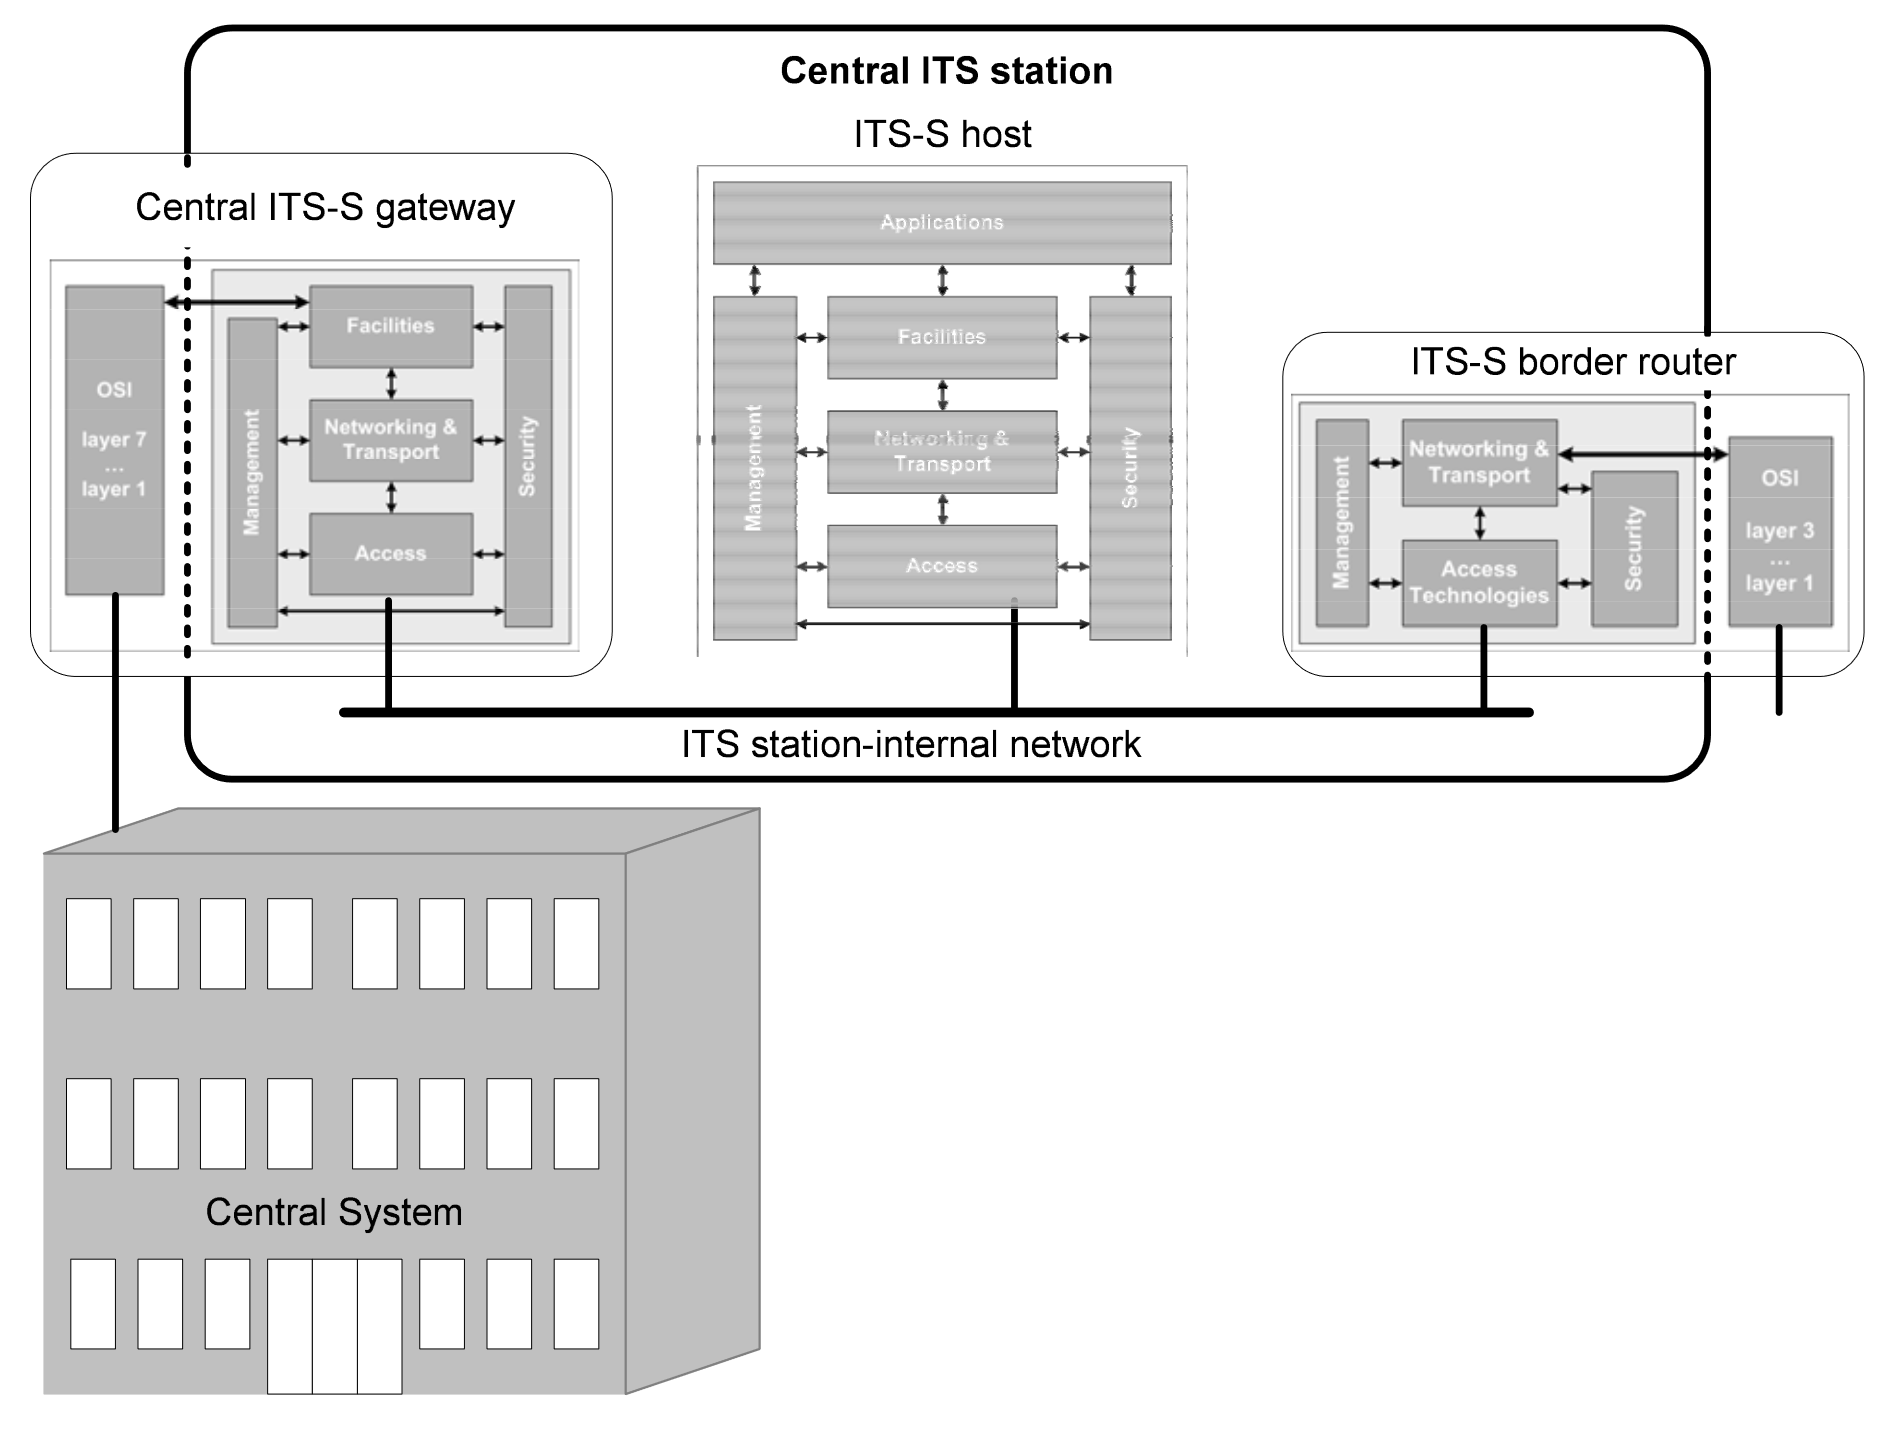
\includegraphics[width=0.8\textwidth]{Chapters/Figures/VANETs/central_ITS.png}
   	\caption{Central \gls{its} station in a Central \gls{its} sub-system~\cite{etsi_intelligent_2010}}
   	\label{fig:central_its}
\end{figure}

The border router communicates with any other \gls{its} system via any external network, while the gateway provides a more standardized connection.
% Vehicle
	\item Vehicle \gls{its} sub-system:

The Vehicle \gls{its} sub-system represents the cars, buses, trains, trucks, airplanes, and any other vehicle or means of transportation that can communicate wirelessly in an ad hoc manner and belongs to the \gls{vanet} space. This definition is very similar to the \gls{obu} definition made by the \gls{c2c}, but there are some important minor differences that make it more rigorous.

This sub-system is made up of the Vehicle \gls{its} station and the internal vehicle network, which is connected to a variety of \glspl{ecu}.
\glspl{ecu} represent any kind of system or application that requires a connection to the Internet or to any other vehicle. Examples of such applications are \gls{gps}, traffic control, road hazard warnings, etc.

Like all stations, the Vehicle \gls{its} station is made up of an \gls{its} host with two optional \gls{its} interceptors, nominally an \gls{its} gateway and an \gls{its} router. This sub-system is depicted in Figure \ref{fig:vehicle_its}.

\begin{figure}[htbp]
    \centering
   	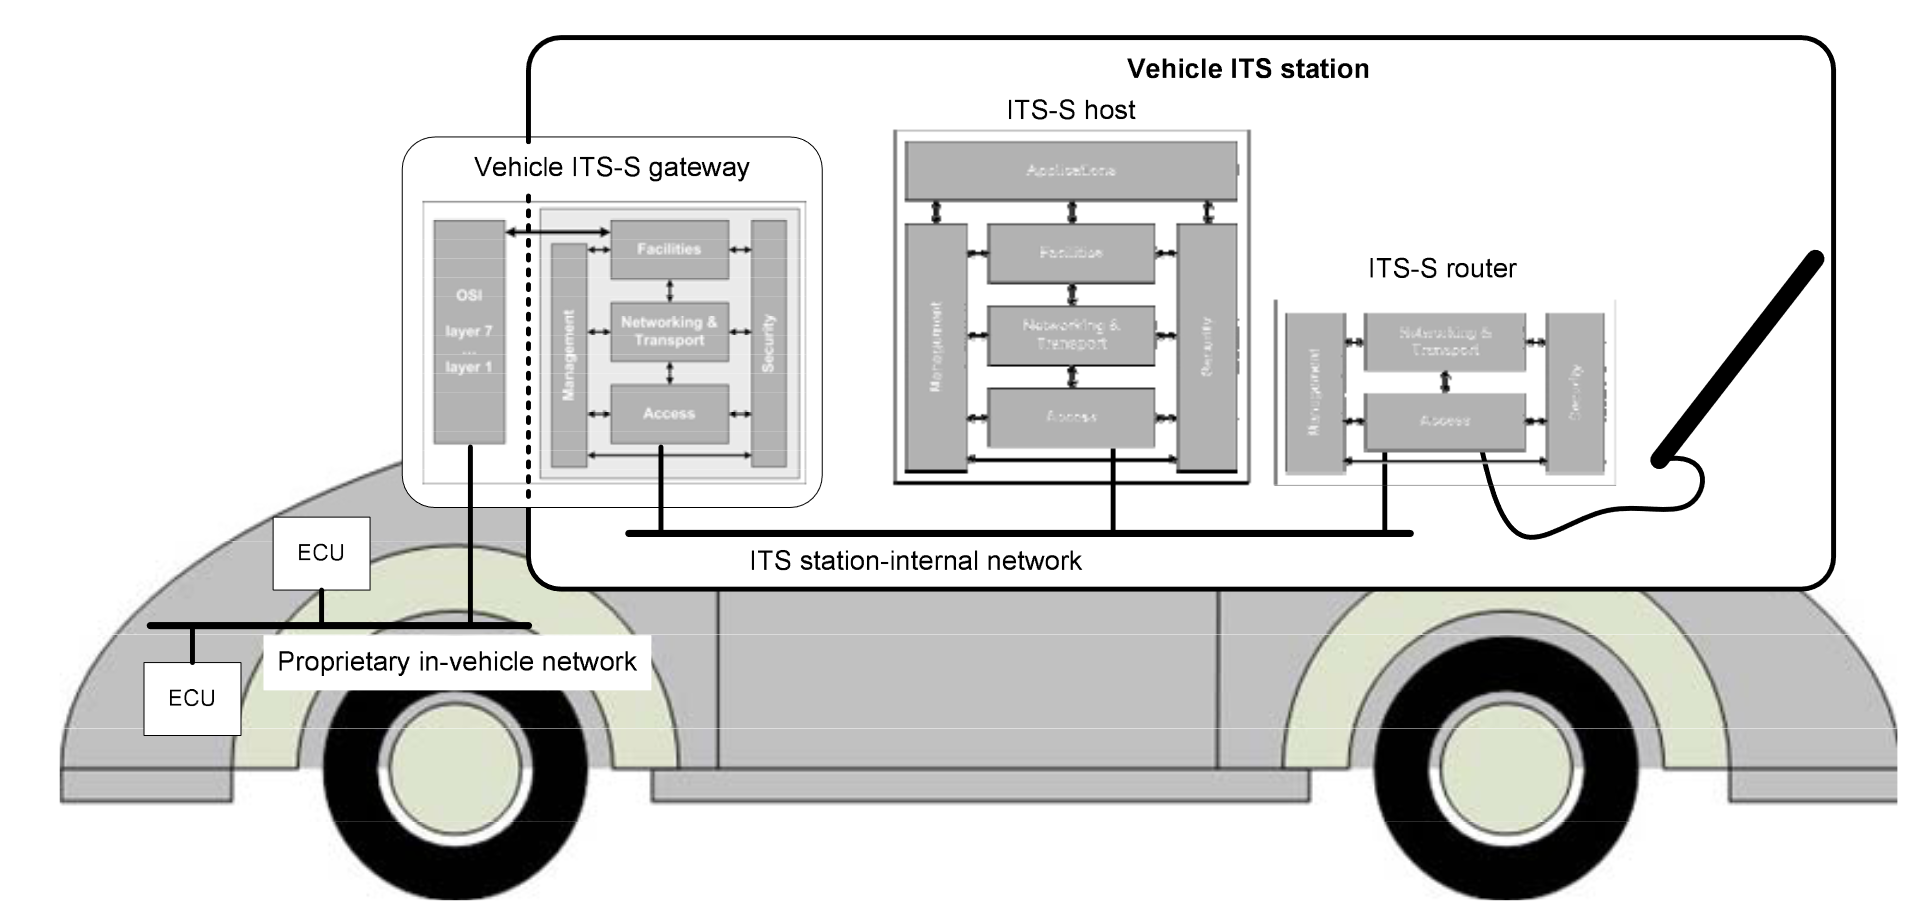
\includegraphics[width=0.8\textwidth]{Chapters/Figures/VANETs/vehicle_ITS.png}
   	\caption{Vehicle \gls{its} station in a Vehicle \gls{its} sub-system~\cite{etsi_intelligent_2010}}
   	\label{fig:vehicle_its}
\end{figure}

The \gls{its} gateway connects the internal vehicle network, which is proprietary in most cases, to the \gls{its} station. Meanwhile, the \gls{its} router connects to other Vehicle \gls{its} stations and, most importantly, to the Roadside \gls{its} station.
        	% Roadside 
\item Roadside \gls{its} sub-system: 

The final element is the Roadside \gls{its} sub-system. It is the connection point between the vehicle ad hoc network and the rest of the Internet. Like the \gls{rsu}, it is placed in locations of high vehicle volume next to roads and intersections.

This sub-system comprises a roadside \gls{its} station and any proprietary roadside network that may exist. It connects to any vehicle \gls{its} station and can provide \gls{its} applications to the vehicle users. This station is also connected to a central \gls{its} station, being the bridge that allows the central \gls{its} station to provide \gls{its} applications to vehicle users.

The roadside station is made up of an \gls{its} host with optional \gls{its} interceptors. These interceptors can be any of the other types of functional components beyond the \gls{its} host. The Roadside \gls{its} sub-system is better depicted in Figure \ref{fig:roadside_its}.

\begin{figure}[htbp]
    \centering
   	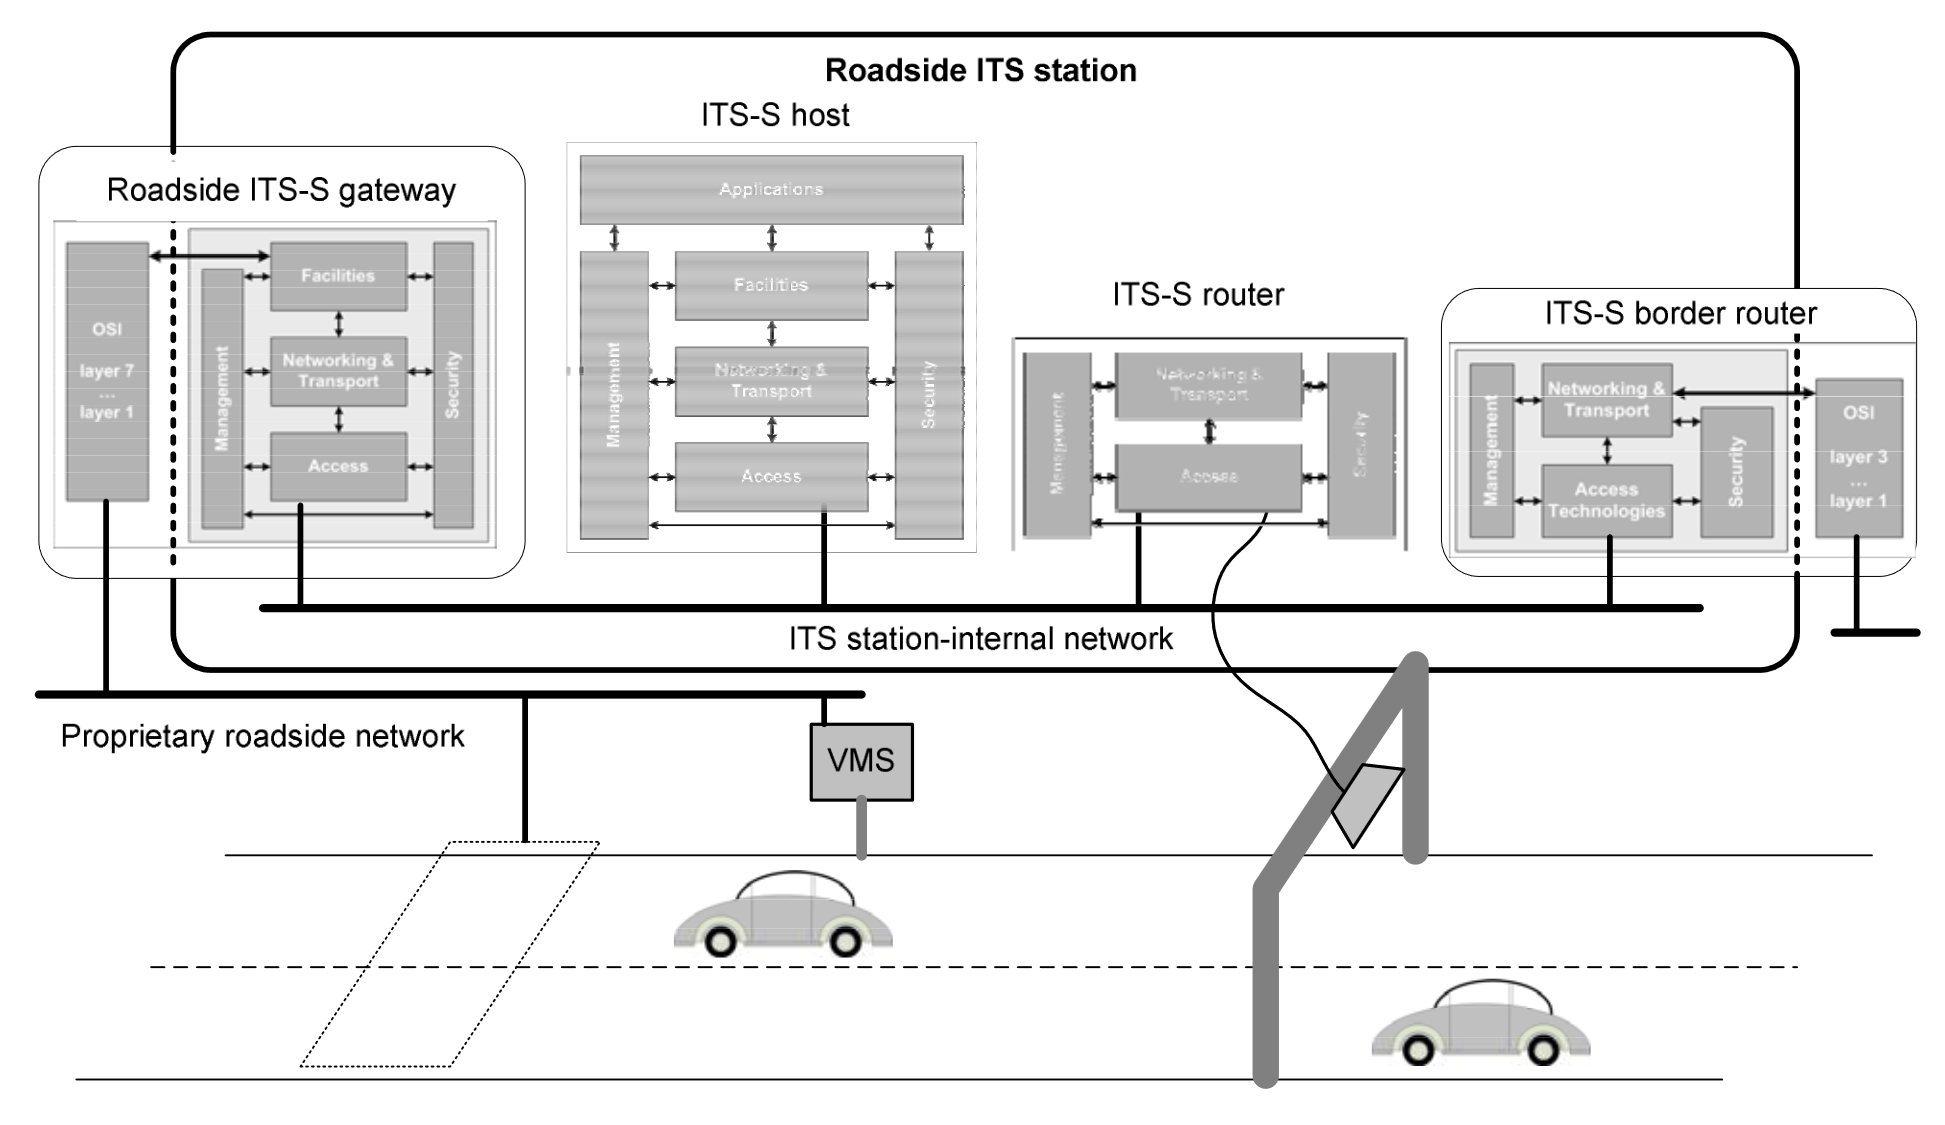
\includegraphics[width=0.8\textwidth]{Chapters/Figures/VANETs/roadside_ITS.png}
   	\caption{Roadside \gls{its} station in a Roadside \gls{its} sub-system~\cite{etsi_intelligent_2010}}
   	\label{fig:roadside_its}
\end{figure}

The \gls{its} router connects the station to the \gls{its} vehicle station, the border router connects to an \gls{its} central station and the gateway connects to any existing proprietary existing networks.

\end{enumerate}


\section{Communication Domains}
\label{sec:VANET_communication_domains}

% Domains
With the main building blocks of both architectures laid out, we can divide communications into various domains. Both the \gls{c2c} and \gls{etsi} have different ways to tackle this question.

\subsection[C2C approach]{\gls{c2c} approach}
% C2C-CC
The \gls{c2c} focuses on the \gls{vanet} space and divides it into three areas: the in-vehicle domain, the ad hoc domain, and the infrastructure domain.
% In-vehicle domain
The first represents the network inside a vehicle, composed of an \gls{obu} and the multitude of \glspl{au} connected to it. It encompasses all communications between the different \glspl{au} and the \gls{obu}.
% Ad hoc domain
The ad hoc domain involves all ad hoc communications between different \glspl{obu} and between vehicles' \glspl{obu} with \glspl{rsu}.
% Infrastructure domain
The remaining components of the Internet that don't directly affect it, but help provide connectivity to vehicles, are included in the Infrastructure domain.

All of these domains, as well as the functional components of the \gls{c2c} architecture can be observed on Figure~\ref{fig:c2c_domain}.

\begin{figure}[htbp]
	\centering
	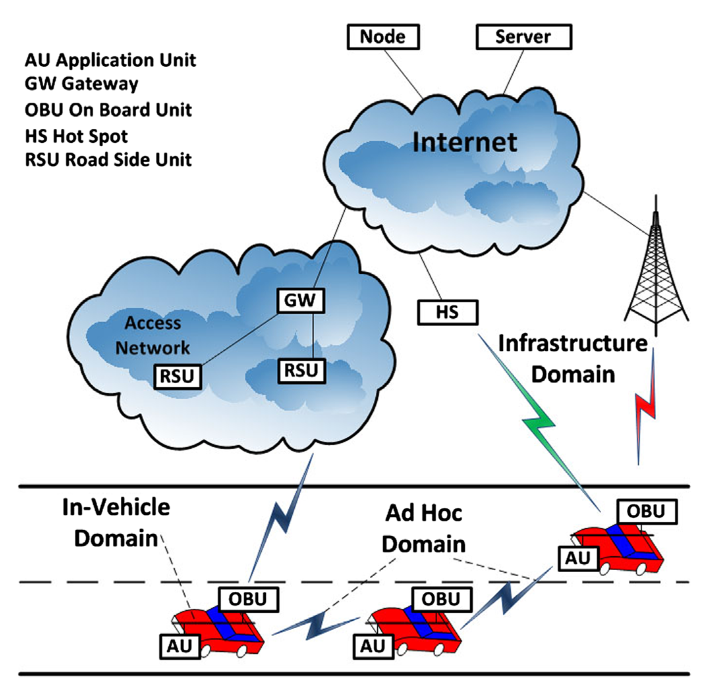
\includegraphics[width=0.8\textwidth]{Chapters/Figures/VANETs/C2C-CC_domains.png}
	\caption{Communication domains in \gls{vanet} as categorized by the \gls{c2c}~\cite{al-sultan_comprehensive_2014}}
	\label{fig:c2c_domain}
\end{figure}

\subsection[ETSI approach]{\gls{etsi} approach}
% ETSI
The \gls{etsi} architecture proposes a broader categorization by establishing two domains. 
%ITS domain
The first and most important is the \gls{its} domain, since it contains all the elements and communication engaged by the \gls{its}/\gls{itsc} standards. 
% Generic domain
Everything else is encompassed by the generic domain, including everything in the rest of the Internet that might interact and communicate with the \gls{its} domain.


\section{Communication categories}
\label{sec:VANET_communication_categories}

% Types of communication (connectivity-oriented architecture)
In addition to communication domains, most authors use a classification based on communication types. This communication-oriented view of architecture aims to classify the multitude of types of communication that can occur between all the different entities that exist.

Different categories have emerged and evolved throughout the years as they have been used by most of the relevant researchers in the field. It is therefore difficult to find an origin for these concepts, and the following are most commonly used terms.

\begin{enumerate}
    % Intra-Vehicle communication
	\item Intra-Vehicle communication
    This term encompasses all communications that occur inside the vehicle between different vehicle components.
    % Vehicle-to-Vehicle (V2V) communication
	\item \gls{v2v} communication
    \gls{v2v} communication refers to the ad hoc communication between vehicles.

    % Vehicle-to-Infrastructure (V2I) communication
	\item \gls{v2i} communication
    \gls{v2i} communication refers to ad hoc communication between vehicles and roadside infrastructure. These communications dont encompass all messages that get exchanged between vehicles and the roadside infrastructure, and only include messages whose source and destination are a vehicle and a roadside station.

    % Vehicle-to-Everything (V2X) communication
	\item \gls{v2x}
    The last type of communication is the most encompassing. \gls{v2x} communication includes all communication that can occur in the \gls{vanet} space between a vehicle and anything else. It is generally used to refer to the previous two types of communication.

\end{enumerate}


\section[VANET architecture]{\gls{vanet} architecture}
\label{sec:vanet_arch}

The architecture of an \gls{its} host can be visualized on Figure \ref{fig:its_host}. This section will dissect this architecture layer by layer in order to explain the functionalities and capabilities expected from it. The last layer, called Applications, will not be described as it represent \gls{its} applications that use the services provided by the rest of the stack to connect one or more applications together and provide services to users~\cite{etsi_intelligent_2010}.

\begin{figure}[htbp]
    \centering
   	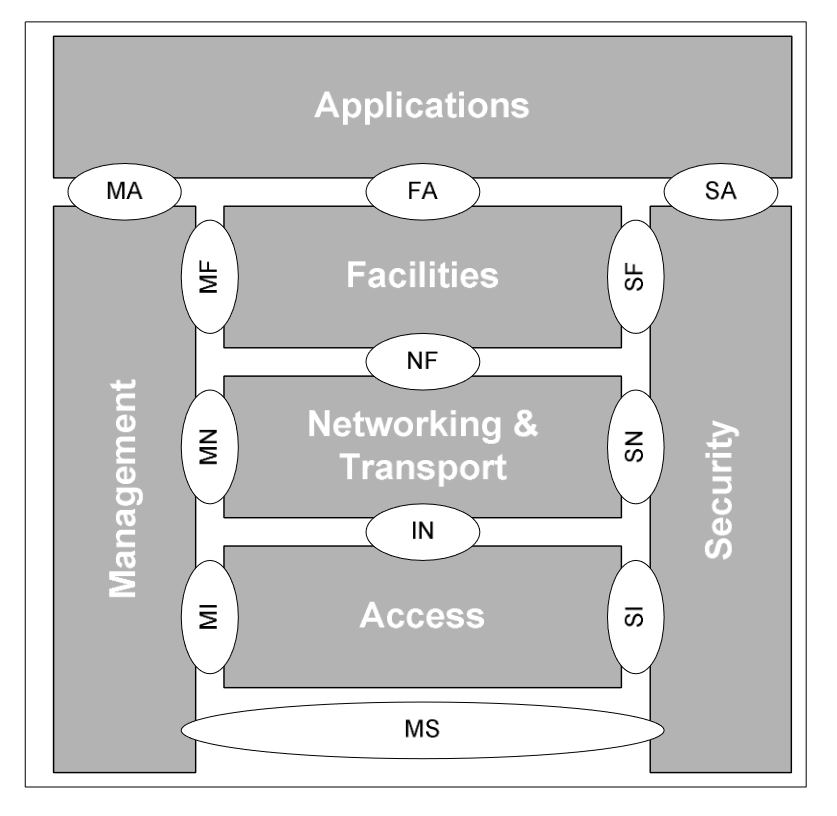
\includegraphics[width=0.8\textwidth]{Chapters/Figures/VANETs/ITS-S_host_arch.png}
    \caption{\gls{its} station reference architecture~\cite{etsi_intelligent_2010}}
   	\label{fig:its_host}
\end{figure}

The functionalities described in every layer are not necessarily function to be implemented in every instance of the architecture, as it depends on the specific implementation of the \gls{its} station~\cite{etsi_intelligent_2010}.

\subsection[Access layer]{Access layer}
\label{subsec:Access_layer}

% Access layer
The Access layer, which is illustrated in the architecture of an \gls{its} host in Figure \ref{fig:its_host}, corresponds to the first two layers of the \gls{osi} model, the Physical layer and the Data link layer~\cite{etsi_intelligent_2020}.

Among all the existing Access layer technologies, the best suited to meet the necessary requirements for use in \glspl{vanet} were the existing wireless access technologies~\cite{al-sultan_comprehensive_2014}. These technologies ranged from long range signaling technologies such as Microwave and WiMAX to short range technologies such as Infrared or Bluetooth~\cite{anwer_survey_2014}.

Over the years, most of these technologies have been studied and tested as possible solutions for use in \gls{vanet} communications, and in most cases they were deemed unsuitable for the \gls{vanet} environment. For instance, short-range communication protocols such as the examples above were discarded due to lack of range, throughput, and reliability and as a result, medium and long range communications took center stage.

While unable to fully address the demanding scenarios of \glspl{vanet}, a few of these technologies showed promise as possible solutions. Over the years since \gls{vanet} research began, new standards and protocols have been developed based on these existing technologies, focusing on solving the problems posed by the characteristics of \glspl{vanet}. In addition, these technologies themselves have evolved to meet the high data rates required by today's Internet.

Today, the \glsxtrshort{ieee} 802.11 WiFi and Cellular technologies are considered as the two primary solutions for \glspl{vanet} worldwide.

\subsubsection[IEEE-based technologies]{\gls{ieee}-based technologies}
% IEEE standards
The \gls{ieee} is an American organization dedicated to promoting innovation and technological excellence for the benefit of humanity. Founded in 1963, it is the world's largest professional society of engineers, scientists, and other technical professionals. \glspl{ieee} primary areas of contribution are the electrical, electronic, and computing fields~\cite{noauthor_history_nodate}.

% IEEE 802.11p
The \gls{ieee} 802.11 family of standards, an Access layer technology, was considered a promising solution for \glspl{vanet} from the start. Not only would the existing \gls{ieee} 802.11 standards be cheaper to adopt due to being already established technologies, but WiFi also already met many \gls{its} requirements due to its compatibility with mobile environments~\cite{rohde__schwarz_intelligent_2019}.

Despite these significant advantages, the existing \gls{ieee} 802.11 standards were not able to meet all the requirements imposed by the unique characteristics of \glspl{vanet}, necessitating the creation of a new variant that would be better suited for such scenarios. Thus, \gls{ieee} 802.11p was created as an adaptation of the existing \gls{ieee} 802.11 standards. Given its American origin and contribution to the development of \gls{v2x} communication technologies, it is important to mention that \gls{ieee} 802.11p was conceived in the context of \gls{wave}~\cite{jiang_ieee_2008}. The \gls{eu}, while initially open to many different access technologies, eventually converged on a \gls{ieee} 802.11p based solution dubbed \gls{its}-G5.

\gls{ieee}'s main motivation behind the development of \gls{ieee} 802.11p was to enable effective communication capable of handling the rapidly changing environments of \glspl{vanet}~\cite{jiang_ieee_2008}, while making the minimum necessary changes to the \gls{ieee} 802.11 Physical layer. Modifying the Physical layer is akin to a software update, while a Physical level amendment would require the design of an entirely new wireless airlink technology~\cite{jiang_ieee_2008}, which would be expensive and time consuming. 

With this in mind, the \gls{ieee} began work on a variant of the \gls{ieee} 802.11 standard that would be feasible for \gls{v2x}, capable of operating at speeds up to 200 km/h and ranges up to 1 km~\cite{jakubiak_state_2008}. Experimental work began with the full deck of \gls{ieee} 802.11 technologies~\cite{toor_vehicle_2008}, but soon narrowed down to \gls{ieee} 802.11a because it operates at 5 GHz, which is closest to 5.9 GHz, the desired frequency for \gls{its} operations in the \gls{us}. This made it easier to configure devices to operate at the desired frequency~\cite{jiang_ieee_2008}.


% Characteristics
% Channel bandwidth
\gls{ieee} 802.11p uses orthogonal frequency division multiplexing. The \gls{ieee} 802.11 family of standards offers three channel bandwidths of 5, 10, and 20 MHz, and while \gls{ieee} 802.11a uses the full 20 MHz bandwidth, the 10 MHz bandwidth was chosen for \gls{its} scenarios. This is achieved either by halving the clock/sampling rate or by simply doubling all the standard orthogonal frequency division multiplexing timing parameters~\cite{rohde__schwarz_intelligent_2019}.

Reducing the channel bandwidth was done in an effort to increase the root mean square delay spread~\cite{toor_vehicle_2008}. Root mean square delay spread measures the time difference in seconds between the first and last signal components. These components represent different versions of the same transmitted signal, with the first to arrive coming from the shortest path which is the light of sight and the remaining coming from reflections and other interactions with the environment.

The standard 20MHz guard used by 11a proved sufficient to stop intersymbol interference between a radio and itself, so measures had to be taken to reduce the interference caused by multipath delays and by the Doppler effect. Halving channels width was the most simple and sensible solution to this problem~\cite{jiang_ieee_2008}. Beyond reducing the signal bandwidth, the data throughput ranges were also reduced to 3 to 27 Mb/s instead of the original 6 to 54 Mb/s~\cite{toor_vehicle_2008}.

% No more BSS
With the goal of enabling effective communications that can cope with rapidly changing environments, \gls{ieee} 802.11p communications needed to get faster in order to better utilize the sometimes narrow windows available for communication. Such a feat demanded a reduction in the overhead required before actual data transmission, which was achieved by simplifying the \gls{bss} operations present in \gls{ieee} 802.11a~\cite{jiang_ieee_2008}.

The \gls{bss} represents a group of stations that are wirelessly connected to the same access point. It is created by an access point, and any device requesting to join it can exchange information with it after proper authorization. A \gls{bss} variant for ad hoc environments exists, called \gls{ibss}, which works without the need for infrastructure. However, it also proved to be insufficient to deal with the peculiarities of \glspl{vanet}.

As a solution, \gls{ieee} 802.11p uses an ad hoc mode called \gls{ocb}. \gls{ocb} simplifies setup operations compared to its counterparts in other \gls{ieee} 802.11 standards by eliminating management procedures such as channel scanning, authentication, and association. This means that \gls{ieee} 802.11p has no setup time allowing stations to communicate with each other directly and immediately~\cite{festag_cooperative_2014}.

Removing all of these processes makes the network less secure. However, these security vulnerabilities are addressed by other standards in the \gls{its} domain.

% Channels
In Europe, \gls{etsi} created a solution for the access layer called \gls{its}-G5. It not only defines the technologies and protocols to be used in communications, but also includes the frequency allocated exclusively for \gls{v2v} and \gls{v2i} communications for the whole of the \gls{eu}.~\cite{asselin-miller_study_2016} \gls{its}-G5 uses the existing \gls{ieee} 802.11p standards created for the American \gls{wave}, adapting it for the European region.

In the \gls{us}, the \gls{fcc} was responsible for the allocation of the frequency from 5.850 to 5.925 in 1999. In 2003, the \gls{fcc} divided the American band into seven non-overlapping 10 MHz channels with a 5 MHz unused band at the lower end. These channels were numbered from 172 to 184. This division also allows for operations in the 20 MHz channels 175 and 181, which are the overlap of two 10 MHz channels~\cite{harri_multi-channel_2015}.

\begin{figure}[htbp]
    \centering
    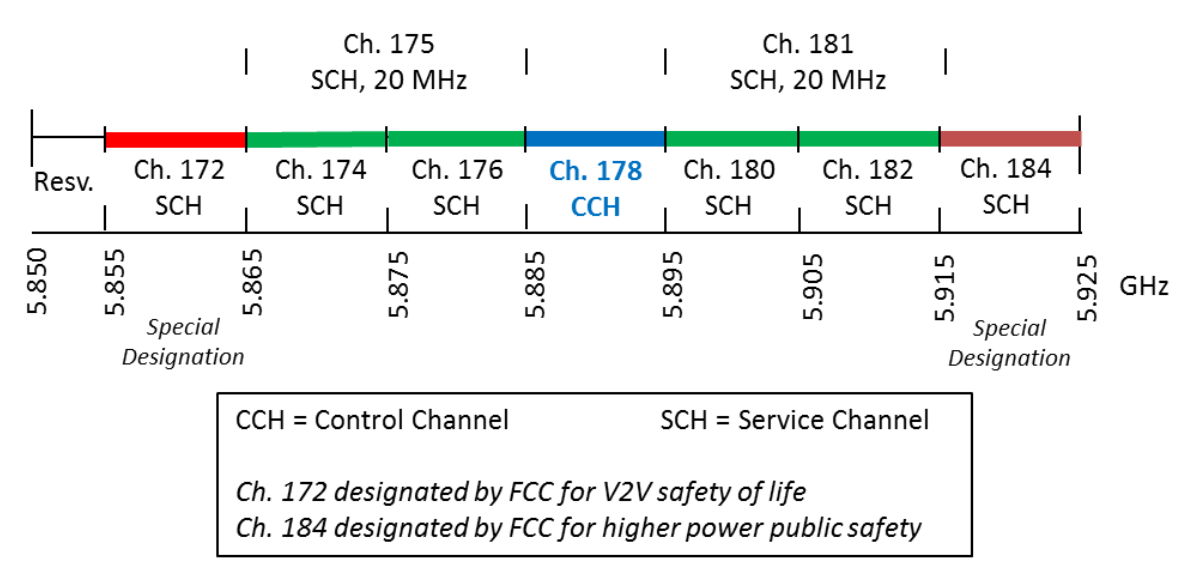
\includegraphics[width=0.8\textwidth]{Chapters/Figures/VANETs/WAVE_channels.png}
   	\caption{Channels allocated in the \gls{us} by \gls{fcc} for \gls{its}~\cite{harri_multi-channel_2015}}
   	\label{fig:WAVE_channels}
\end{figure}

In the \gls{eu}, the \gls{ecc} is responsible for spectrum regulation and the European Commission is responsible for enforcing the regulated spectrum in all member states. The \gls{ecc} is made up of radio and telecommunications regulatory authorities from all member countries~\cite{harri_multi-channel_2015}~\cite{asselin-miller_study_2016}.

The spectrum allocation for \gls{its}-G5 began in 2005, with a recommendation from \gls{etsi} to the \gls{ecc}. In its TR 102 492-1~\cite{etsi_electromagnetic_2005}, \gls{etsi} recommended the allocation of 30 MHz in the 5,875 GHz to 5,905 GHz band for safety applications, which would align with the \gls{us} control channel frequency of 5,885 GHz to 5,895 GHz. This recommendation also expected the allocation of a future 20 MHz band from 5,905 GHz to 5,925 GHz for future \gls{its} extensions~\cite{harri_multi-channel_2015}~\cite{asselin-miller_study_2016}.

\gls{etsi} based this recommendation on the allocation in the \gls{us} frequency band, and also took into account the 5.8GHz toll collection band used in \gls{eu} countries~\cite{harri_multi-channel_2015}~\cite{asselin-miller_study_2016}.

In 2008, the \gls{ecc} accepted this recommendation and allocated the requested frequency range plus another 20 MHz frequency band from from 9,855GHz to 9.875GHz intended to be used by non-safety applications~\cite{harri_multi-channel_2015}~\cite{asselin-miller_study_2016}. All of the spectrum involved for present and future \gls{its} operations can be easily observer in Figure \ref{fig:EU_channels}.

\begin{figure}[htbp]
    \centering
    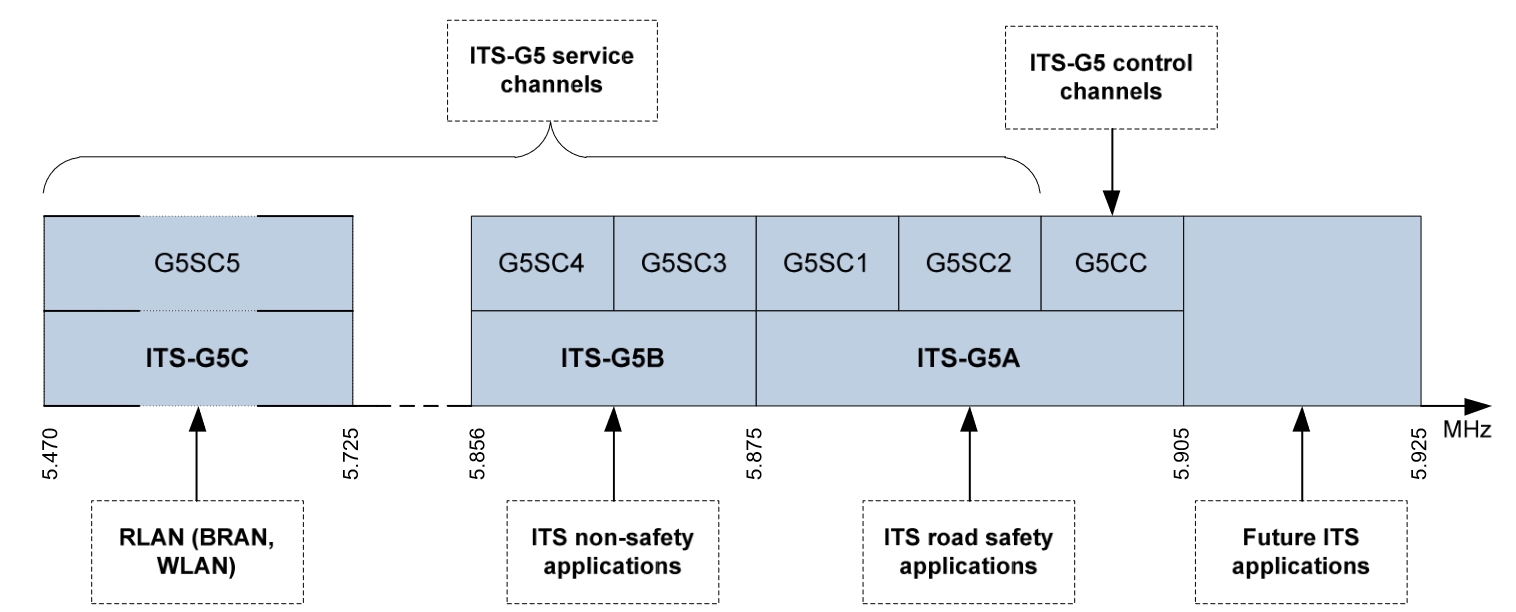
\includegraphics[width=0.8\textwidth]{Chapters/Figures/VANETs/European_its_channels.png}
   	\caption{European \gls{its} channel allocation~\cite{soriga_its-g5_2012}}
   	\label{fig:EU_channels}
\end{figure}

Even though the American spectrum was taken into consideration, in the end the control channels of both the \gls{eu} and \gls{us} solutions were not in the same frequency, with the European channel being 10 MHz higher. This is not a total loss, as the same hardware can still be used in both countries requiring just a software change to work~\cite{harri_multi-channel_2015}~\cite{asselin-miller_study_2016}.

The different allocated frequencies have different standardized transmission power limits based on use cases and interferences on adjacent bands and on the more important control bands~\cite{festag_cooperative_2014}. The specific restrictions for each 10 MHz channel can be observed in figure \ref{fig:EU_channet_restriction}.

\begin{figure}[htbp]
    \centering
    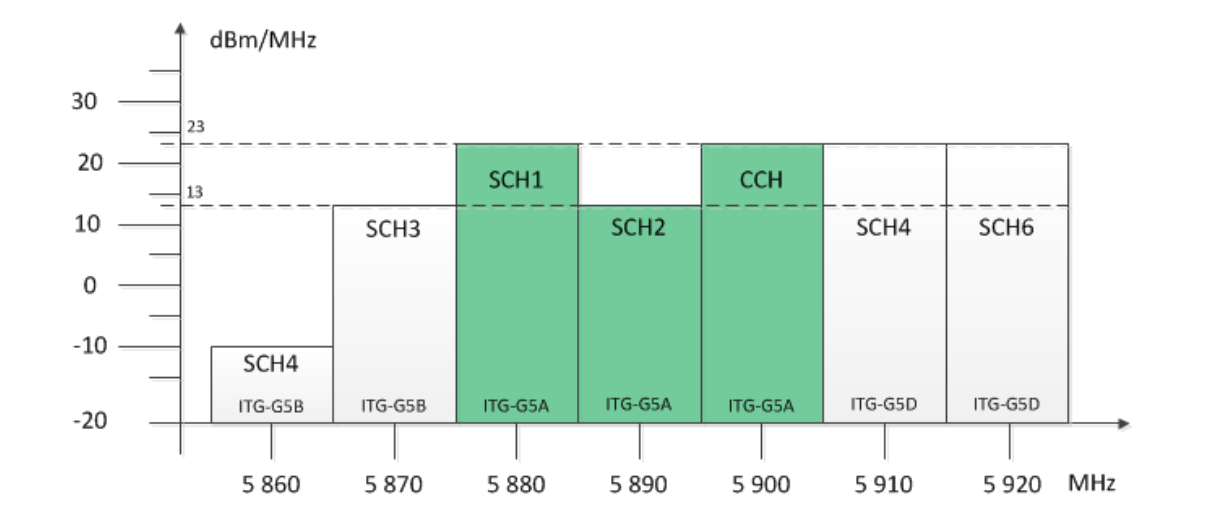
\includegraphics[width=0.8\textwidth]{Chapters/Figures/VANETs/European_its_channels_restrictions.png}
   	\caption{Power spectral limits on each \gls{its} channel~\cite{harri_multi-channel_2015}}
   	\label{fig:EU_channet_restriction}
\end{figure}

% IEEE 802.11bd
In recent years, the \gls{ieee} began work on \gls{ieee} 802.11bd, a successor to the \gls{ieee} 802.11p standard, which was approved in October 2023~\cite{noauthor_ieee_2023}. As a new standard, it is expected to take several years before it completely replaces 11p, and most automakers will continue to release cars with \gls{ieee} 802.11p for the foreseeable future.

This new version promises twice the throughput and longer range, while ensuring interoperability, coexistence, backward compatibility and fairness with existing \gls{ocb} terminals. In addition, it operates beyond the 5.9 GHz band by utilizing the 60 GHz band.


\subsubsection{Cellular-based technologies}
% Cellular-based communication in VANETs
Cellular systems have been used since the 1970s to transmit data over long distances via radio waves~\cite{anwer_survey_2014}. The \gls{3gpp} is an international consortium established in 1980 with the goal of developing technical specifications and technical reports for 3G mobile systems and is now the leading global reference for mobile standards and is responsible for the development of \gls{lte} and 5G~\cite{noauthor_3gpp_nodate}.

Although most work on \glspl{vanet} has been based on \gls{ieee} 802.11p, \gls{c-v2x} has gained renewed support from academia and industry as this technology has matured~\cite{gyawali_challenges_2021}. Rival performance to the dominant \gls{ieee} 802.11p has led to Cellular technologies being considered by some organizations as a replacement for existing \gls{ieee} standards, so its status as the second most important \gls{vanet} technology is not surprising.

In September 2016, the \gls{5gaa} was established as a global, cross-industry organization of companies from the automotive, technology, and telecommunications industries with its main objective to promote the use of cellular \gls{3gpp} standards in \gls{its} scenarios~\cite{noauthor_5gaa_nodate}.

% Drawbacks and Benefits for C-V2X
Most researchers dismissed this new technology because its shortcomings made it seem inadequate compared to the strengths of \gls{ieee} 802.11. \gls{c-v2x}'s main drawback is its centralized nature. Cellular technology relies on a centralized infrastructure, which introduces latency by forcing all data to pass through a base station.

In addition, the large coverage area of cellular antennas can also pose an issue, as the coverage area of an antenna is typically larger than the zone of relevance of safety messages. This makes broadcast an inadequate solution, as many vehicles would receive warnings not intended for them. Multicast can be introduced in an attempt to reduce this problem, but it introduces new delays from the overhead required to create these multicast groups~\cite{gyawali_challenges_2021}.

On the other hand, Cellular technologies have several technical and economic advantages for their application in \gls{v2x} communications. On the technical side, cellular technologies provide wide coverage, support high vehicle speeds, support a large number of connections to a single cell tower and can deliver high data rates. Economically, the wide use of these technologies allows the reuse of already deployed hardware for use in \gls{v2x}~\cite{gyawali_challenges_2021}.

% LTE/5G
These benefits, along with the renewed support from the industry created from \gls{5gaa}, motivated the \gls{3gpp} to begin studying the feasibility of \gls{lte} technology for supporting \gls{v2x} communications~\cite{gyawali_challenges_2021}. In 2019, \gls{3gpp} began work on \gls{c-v2x} efforts with Release 14, which made great strides in reducing existing drawbacks.

In order to work as a wireless access technology capable of serving all \gls{vanet} test cases, this technology needed to ditch the necessity of using infrastructure and become ad hoc. Therefore, Release 14 established a new mode of communication, called direct communication.~\cite{weber_c-v2x_2019} This resulted in \gls{lte} and 5G supporting two relevant interfaces for communication in \glspl{vanet}, the Uu interface and the PC5 interface.

The Uu interface is used for long range communication with cellular infrastructure in the commercial cellular spectrum. It uses existing \gls{lte}'s large coverage to provide vehicles with all kinds of services~\cite{weber_c-v2x_2019}.

The direct communication mode, also referred to as “Mode 4”, utilizes the short range PC5 interface in the \gls{its} 5.9GHz band and allows for direct exchange of information between vehicles without passing through a cell tower.

% Place in standards

\gls{etsi} initially considered Cellular technologies as possible solutions, and at that time included 2G and 3G as possible access technologies in the initial \gls{its} station reference architecture. As stated earlier, \gls{etsi} centralized the Access layer of its architecture on the \gls{ieee} 802.11p-based \gls{its}-G5. Recently, however, reflecting on the efforts of \gls{3gpp}, \gls{5gaa}, and \gls{its} implementation in other countries like China, \gls{etsi} made amendments to existing standards in order to achieve compatibility with \gls{c-v2x} technologies~\cite{weber_c-v2x_2019}. This indicates that in the \gls{c-v2x} architecture, the layers above the Access layer consists of the pre-established standards of different countries, demonstrating significant technological compatibility.


\subsection[Networking \& Transport layers]{Networking \& Transport layers}
\label{subsec:networking_transport_layers}
% Introduction
The Networking and Transport layer, as implied by its name, corresponds to the third and fourth layers of the \gls{osi} model.

% Routing challenges and opportunities in VANETs
layer 3 algorithms commonly deployed in traditional networks are unsuitable for use in \glspl{vanet}~\cite{toor_vehicle_2008}, and even existing \glspl{manet} algorithms have proven to be inadequate for use in \glspl{vanet}~\cite{liang_vehicular_2015}. The characteristics of \glspl{vanet}, as described in section \ref{sec:VANET_characteristics}, present several unique challenges not only to existing layer 3 algorithms, but also to Layer 4 protocols, the most important of which are high node mobility and variable node density.

The high mobility of nodes leads to frequent topology partitions, which results in highly unstable routes. Therefore, pre-determining routes in these conditions is often irrelevant and extremely complicated. Additionally, the algorithm must operate under conditions of both extreme congestion and isolation due to variable node density, further increasing its complexity.

Scholars have recognized the adoption of broadcast as the primary communication mode as a great solution to mitigate interference in high congestion scenarios. Nevertheless, this approach alone falls short of the desired outcome. For instance, in case of a crash, it is essential to rapidly disseminate security messages as the number of affected vehicles can rapidly rise. However, if every vehicle broadcasts simultaneously, it will lead to channel congestion, making it more difficult for the event to spread~\cite{toor_vehicle_2008}. Therefore, novel approaches are required to curb message duplicates. 

Although the challenges presented by these aspects of \glspl{vanet} affect algorithm reliability, researchers have leveraged other characteristics of \glspl{vanet} to develop novel solutions to the aforementioned problems. Besides the lack of power constraints, the predictable mobility of nodes allows algorithms to perform more effective link selection, which facilitates network management and opens opportunities to optimize the flow of information, ultimately improving routing protocols.

% ETSI solution
In Europe, researchers at \gls{etsi} developed new algorithms and defined new protocols in an attempt to find an adequate solution to the aforementioned challenges while taking advantage of \glspl{vanet} newfound opportunities. As part of its architecture, \gls{etsi} introduced a new layer 3 protocol called GeoNetworking~\cite{etsi_intelligent_2014-1}~\cite{etsi_intelligent_2013-1}~\cite{etsi_intelligent_2014}~\cite{etsi_intelligent_2020-1}~\cite{etsi_intelligent_2019}~\cite{etsi_intelligent_2014-2}, a new layer 4 protocol called \gls{btp}~\cite{etsi_intelligent_2019} and a sublayer 3 extension called \gls{gn6}~\cite{etsi_intelligent_2014-2}.

% GeoNetworking 
GeoNetworking is an ad hoc routing protocol that was developed solely for the transmission of safety related messages and therefore it provides the ability to forward packets without the need to exchange any signaling messages beforehand.

The GeoNetworking protocol uses the geographical coordinates of nodes as their address and utilizes location-based data to help make packet forwarding decisions. 

By using a device's geographic location as its address, this protocol enables packets to be sent to all nodes within a specific geographical area. Nodes can effortlessly broadcast messages to an entire geometrically shaped area without congesting the entire network. This approach proves to be more efficient than broadcasting because it curbs congestion by minimizing transmissions to unintended destinations. Moreover, it makes the packet relevance area independent of the sender's range.

This protocol was built and optimized for multi-hop communication with geo-addressing, providing more technical features in application support than the alternative in the \gls{us}. These capabilities come to a cost to protocol complexity and message overhead~\cite{festag_standards_2015}.

% BTP 
The GeoNetworking protocol was designed to be integrated with the \gls{btp} protocol. \gls{btp} is a transport layer protocol that is similar in function to \gls{udp}, functioning as a connectionless protocol~\cite{festag_cooperative_2014}.

% GN6 & IPv6
\gls{etsi} has established the GeoNetworking extension \gls{gn6} as an alternative to routing packets through \gls{btp}. By using the \gls{gn6} sub-layer, \gls{ipv6} packets can be transmitted over the GeoNetworking protocol without the need to modify the \gls{ipv6} protocol~\cite{festag_cooperative_2014}.


\subsection[Facilities layer]{Facilities layer}
\label{subsec:Facilities}

% Facilities layer
% Introduction 
The Facilities layer encompasses layers 5, 6, and 7 of the \gls{osi} model, and its standardization defines application-specific functionalities~\cite{festag_standards_2015}. The development of Facility layer messages is the responsibility of European institutions such as \gls{etsi}, \gls{cen}, and \gls{iso}.

All the messages defined by European standard makers serve safety purposes, and therefore run over the GeoNetworking protocol~\cite{festag_standards_2015}. Multiple different messages have been defined over the years~\cite{festag_cooperative_2014}, which makes it difficult to list them all. However, \glsxtrshortpl{cam} and \glsxtrshortpl{denm} are universally acknowledged as the most significant in the context of \gls{its}.

% CAMs
A \gls{cam}~\cite{etsi_intelligent_2019-2} is a periodic safety message that contains vital status information about the originating vehicle, with the main goal of enabling other vehicles to take appropriate preemptive measures to avoid potentially dangerous situations~\cite{al-sultan_comprehensive_2014}.

This objective is accomplished by exchanging data, including speed, location, direction, and additional non-safety application data with nearby \gls{its} stations, allowing vehicles to monitor each other's movements.~\cite{festag_standards_2015}.

\glspl{cam} begin transmitting as soon as the vehicle enters a safety-relevant context, which is considered to be anytime the vehicle is in operation.~\cite{festag_cooperative_2014} The transmission rate of \glspl{cam} is subject to specific rules, including both maximum and minimum transmission times between \glspl{cam}, relevant changes in position, direction, or velocity, and congestion in the wireless channel~\cite{festag_cooperative_2014}.

\gls{cam} fields are shown in figure \ref{fig:cam_structure}. It includes an obligatory \gls{its} \gls{pdu} header, Basic container, and High frequency container, along with optional Low frequency and Special vehicle containers.

\begin{figure}[htbp]
    \centering
    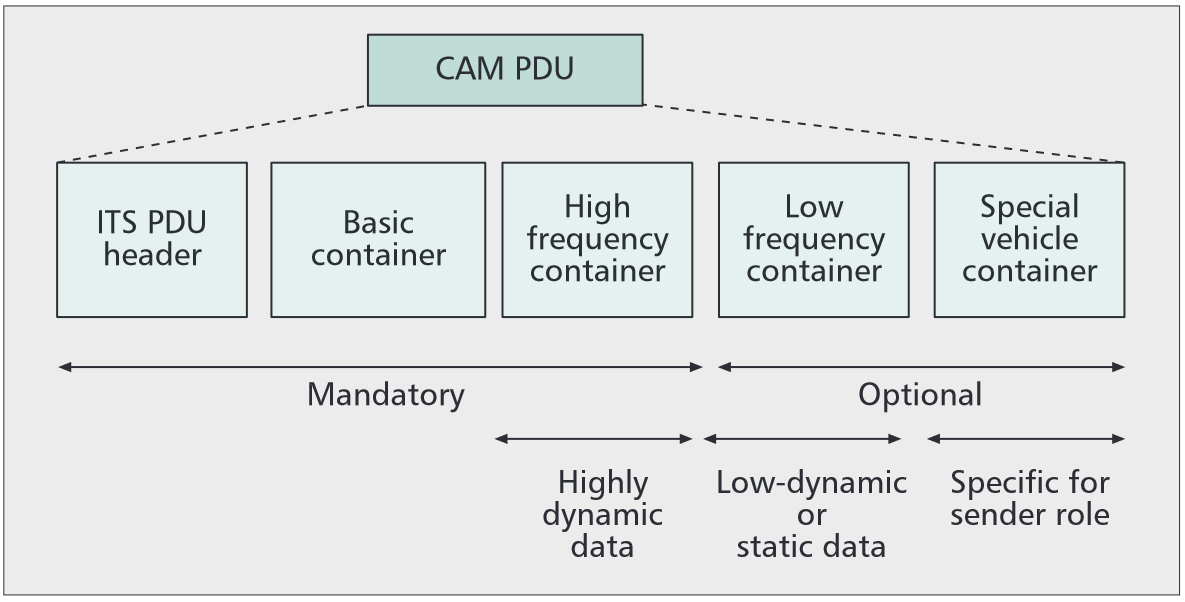
\includegraphics[width=0.8\textwidth]{Chapters/Figures/VANETs/cam_structure.png}
   	\caption{\gls{cam} structure~\cite{festag_cooperative_2014}}
   	\label{fig:cam_structure}
\end{figure}

This structure allows for a high degree of flexibility in message format, allowing messages to adapt more effectively to their environment, thereby minimizing congestion on wireless channels~\cite{festag_cooperative_2014}.

% DEMMs 
A \gls{denm}~\cite{etsi_intelligent_2019-1} is an event-driven safety message that can be triggered by an \gls{its} station in the event that hazardous conditions are detected. \gls{its} stations are capable of detecting a wide range of events and this message type is employed to describe such events to other \gls{its} applications. 

\glspl{denm} serve the purpose of warning \gls{its} applications to a detected event within a designated geographical area~\cite{festag_cooperative_2014}. This type of messages are only relevant in a specific location and therefore are only disseminated in that specific geographical area. These geographical areas are the ones defined by the GeoNetworking protocol.

As an event-triggered message, \glspl{denm} are considered high-priority messages, as ensuring a quick delivery is crucial to diminishing the consequences of the events that triggered their generation~\cite{al-sultan_comprehensive_2014}.

Throughout the lifespan of the \gls{denm}, a number of techniques are employed to ensure the dissemination of the message in its relevant area. \glspl{denm} are repeated, generally at a lower frequency than \glspl{cam}, with the intent to allow vehicles entering the relevant area to receive said information. Similarly, if the originator ceases to transmit the \gls{denm} message for any reason, another \gls{its} station can replace the originator and continue to transmit the message. \gls{denm} messages can also be canceled by the \gls{its} station that created them~\cite{festag_cooperative_2014}.

\gls{denm} fields can be observed on figure \ref{fig:denm_structure}. The \gls{its} \gls{pdu} header and the management container are mandatory, while the situation, location and a la carte container are all optional. These message fields mainly contain information about the relevance area of the message, the type of event and the time in which the message remains relevant.~\cite{al-sultan_comprehensive_2014}

\begin{figure}[htbp]
    \centering
    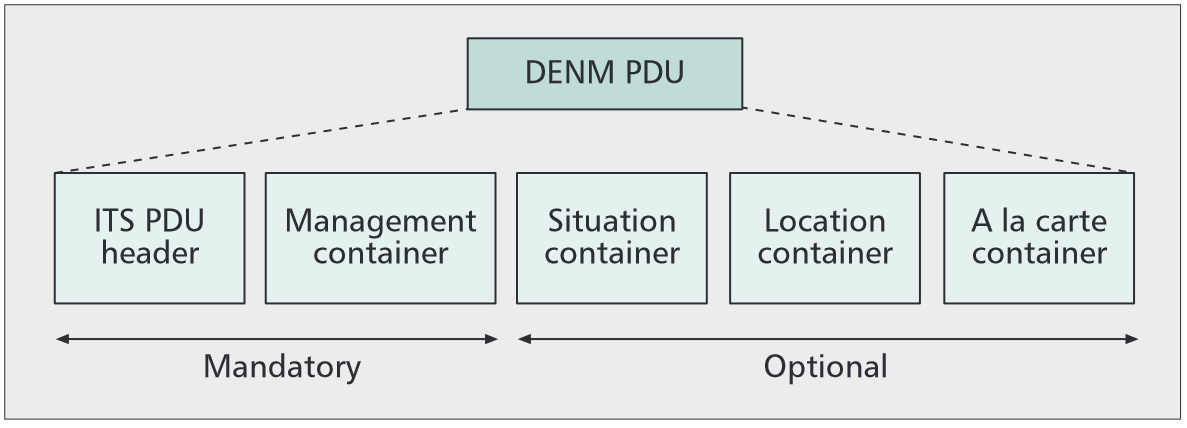
\includegraphics[width=0.8\textwidth]{Chapters/Figures/VANETs/denm_structure.png}
   	\caption{\gls{denm} structure~\cite{festag_cooperative_2014}}
   	\label{fig:denm_structure}
\end{figure}


\subsection[Management Entity]{Management Entity}
\label{subsec:Security_of_VANETs}
% Management
Network management is a critical component of network maintenance as it ensures that a network operates as intended. The unique challenges presented by \glspl{vanet} contribute to a significantly more unstable network environment than usual, making management even more essential. With this motivation in mind, \gls{etsi} incorporated a management entity into its architecture \ref{fig:management_entity}.

\begin{figure}[htbp]
\centering
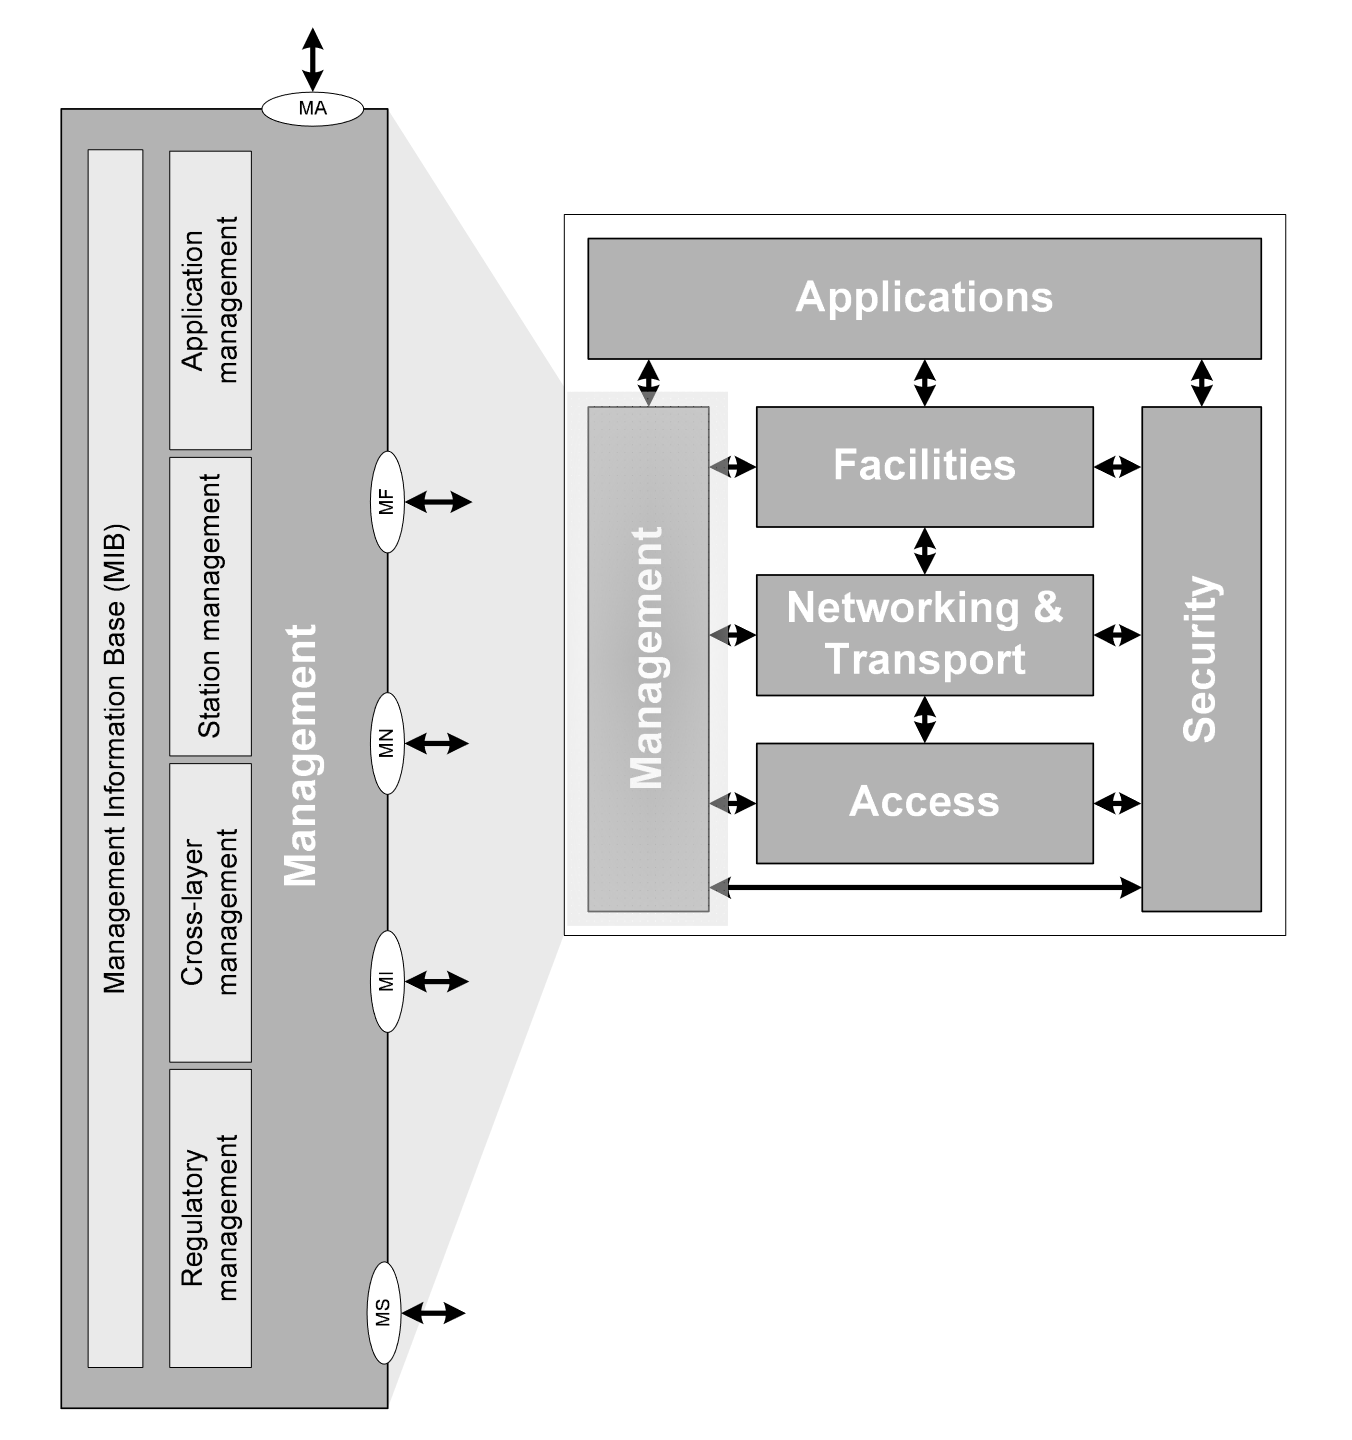
\includegraphics[width=0.8\textwidth]{Chapters/Figures/VANETs/management_entity.png}
   	\caption{\gls{itsc} management entity as part of the \gls{its} station reference architecture~\cite{etsi_intelligent_2010}}
   	\label{fig:management_entity}
\end{figure}


The \gls{its} management entity is responsible for both configuring and operating its \gls{its} station, while also overseeing cross-layer information exchange between multiple layers. It contains interfaces to every other component in the \gls{its} station and a management information base~\cite{etsi_intelligent_2014}. 

Decentralized congestion control is a cross-layer \gls{its} functionality that is coordinated by the management entity and is one of its most important responsibilities. Its main purpose is to control congestion in the channel by managing the amount of messages exchanged, the transmission power and any other useful parameter. The changes to these parameters, being orchestrated by the management entity, are made based on various information extracted from different layers~\cite{festag_cooperative_2014}.



\subsection[Security Entity]{Security Entity}

% Security 
Security in \glspl{vanet} has been one of the biggest concerns and one of the biggest obstacles to its deployment. It is crucial to protect the \gls{its} domain from malicious attacks and network abuse, and as such it has been a high priority for researchers and developers to address security threats prior to deployment.
Vehicle messages can contain a large amount of sensitive information, such as vehicle trajectory and location data. This information can be used to deduce the driver's identity, activities, habits, and so on. This type of information must not only be kept private under \gls{eu} law, but could also be used by bad actors for extortion~\cite{liang_vehicular_2015}~\cite{malhi_security_2020}.
Attackers could also exploit safety messages for their own benefit or to the detriment of others. For instance, greedy drivers could broadcast false traffic alerts to reduce traffic on their own routes. In a more extreme case, robbers or terrorists could abuse traffic alerts to clog roads and thereby delay emergency vehicles~\cite{malhi_security_2020}. 
With this motivation in mind, researchers have laid out several security requirements \glspl{vanet} must meet. The following list contains the most important ones, based on the works of~\cite{hasrouny_vanet_2017}~\cite{malhi_security_2020}:
\begin{enumerate}
	\item Authentication: this security requirement ensures that a recipient can identify the sender of all messages received, thereby ensuring that each message is generated by an authenticated user.
    \item Non-repudiation: sometimes called auditability, it is a tricky to enforce but essential security requirement. Non-repudiation ensures that once a message is sent, the sender can't deny ownership of the message. In \glspl{vanet}, this requirement is essential for identifying compromised users.
    \item Integrity: this security requirement ensures that the message remains unchanged during transmission.
	\item Confidentiality: a security requirement for any type of network, and \gls{vanet} is no different. Some messages contain important information and therefore should only be accessible to the sender and receiver to prevent eavesdropping.
	\item Availability: one of the most important concerns in \glspl{vanet}, this requirement seeks to ensure the availability of the wireless channel, as a message that is delayed by seconds becomes useless.
	\item Access control: this property creates different levels of access for different entities. Access control bars users from accessing any information or sending message types they are not allowed to. Distinguishing multiple levels of access allows for a higher degree of network control and is essential to stop known bad actors from exploiting network dynamics.
	\item Privacy: Privacy is the ability of users to hide their personal information from the rest of network users. Implementing mechanisms to protect the privacy of all drivers is a top priority to ensure driver privacy, with the main goal to provide location privacy. Anonymity is the process of hiding one's identity, which is extremely important to achieve privacy.
	\item Data verification: this property is essential to avoid false messaging as it allows all messages to be tested by their time relevance. This is necessary to avoid replay attacks in the network.
	\item Physical Security: as vehicles are a widely spread technology that will be distributed indiscriminately, it is important to implement hardware security in order to avoid tampering and compromising of the vehicle.
\end{enumerate}
Authentication and privacy are desirable properties of \glspl{vanet} but ensuring anonymity while enforcing network liability in \glspl{vanet} is a contradictory property in securing vehicular networks. This comes from the necessity to protect drivers' privacy while being able to track down attackers~\cite{jiang_ieee_2008}~\cite{malhi_security_2020}. 
Another important consideration to take is that security measures can create performance problems, as they add overhead time in communications and can significantly degrade message quality~\cite{toor_vehicle_2008}. 
	% ETSI security entity
%\gls{etsi} has taken these security concerns into consideration and has incorporated security requirements into its architecture\ref{fig:security_entity}. These considerations were taken on a layer by layer approach, resulting in security services being implemented at every layer and between multiple layers, which necessitated the creation of a dedicated entity for security. The \gls{etsi} \gls{its} host architecture envisions a Security Entity, which is responsible for providing security services, as seen on figure 25. The security entity can also be considered as a specific part of the management entity.
%\cite{etsi_intelligent_2010-1}


\begin{figure}[htbp]
    \centering
    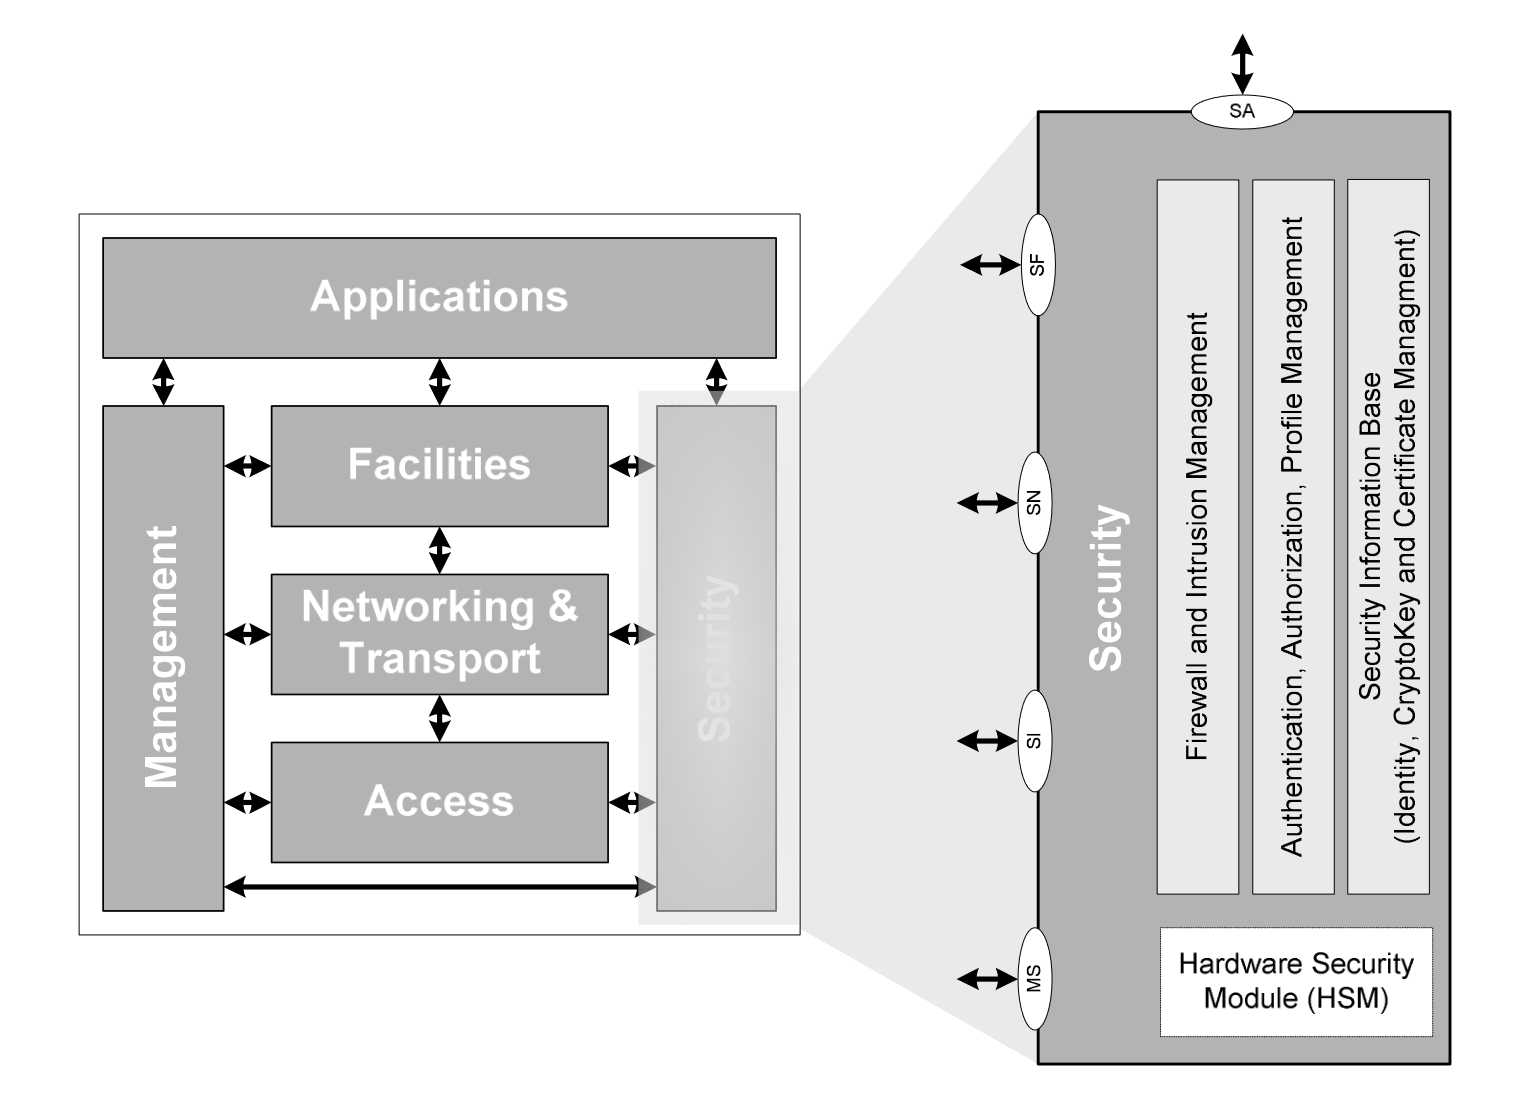
\includegraphics[width=0.8\textwidth]{Chapters/Figures/VANETs/security_entity.png}
   	\caption{\gls{itsc} security entity as part of the \gls{its} station reference architecture~\cite{etsi_intelligent_2010}}
   	\label{fig:security_entity}
\end{figure}


The Security Entity provides a plethora of services to ensure security and privacy. These include a multitude of secure messages at different layers of the communication stack, management of identities and security credentials, and other aspects relevant to secure platforms such as firewalls, security gateways, and tamper-proof hardware~\cite{etsi_intelligent_2014}.


% Authority hierarchy
\gls{etsi} developed an \gls{its} communication system that relies on indirect trust relationships, which are built upon trusted third party certificates. It is a solution to the privacy problem and results in the implementation of a so-called authority hierarchy. This hierarchy is composed of manufacturers, enrolment authorities, authorizations authorities and the \gls{its} station.

\begin{figure}[htbp]
    \centering
    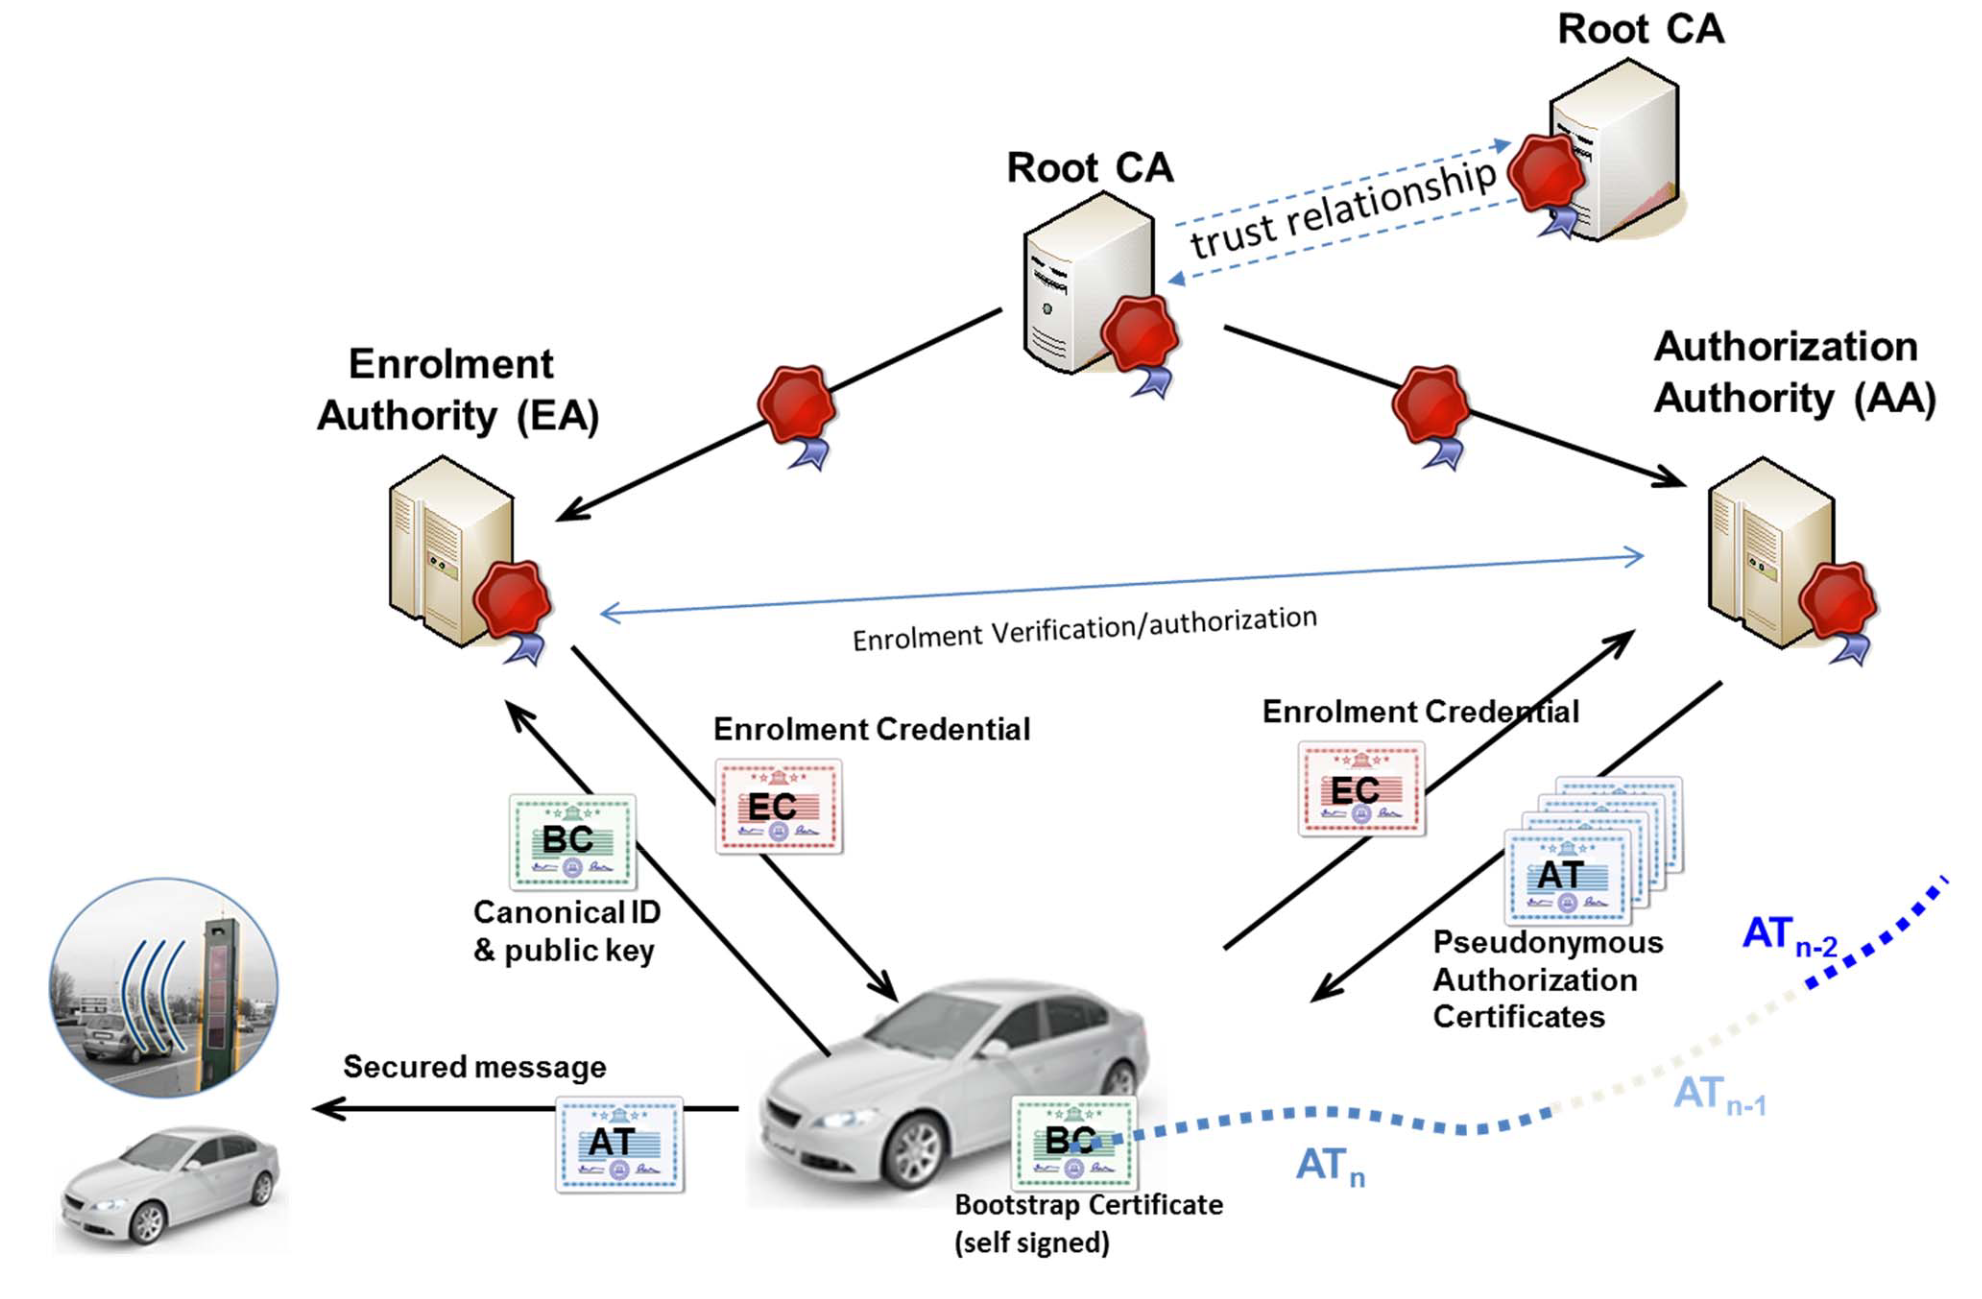
\includegraphics[width=0.8\textwidth]{Chapters/Figures/VANETs/pki.png}
   	\caption{\gls{its} Security Certificate Management System~\cite{etsi_intelligent_2018}}
   	\label{fig:pki}
\end{figure}


When a car wishes to begin communicating, it must use its canonical credentials given by the manufacturer to request valid enrolment credentials to an enrolment authority. Then, using the enrolment credentials it must request an authorization authority for authorization credentials. These last ones are the ones that will be used for communications, and as such in order to protect a driver's privacy are only valid in a time frame. After these expire, the \gls{its} host must request new authorization credentials to the authorization authority.
From this example, we can observe that the enrollment authority validates that the vehicle has a valid \gls{its} station and that the authorization authority uses the authorizations given by the enrollment authority to allow the \gls{its} station access to the \gls{its} domain and to utilize a specific type of applications, service or privilege. This process can be observed on Figure \ref{fig:pki}~\cite{etsi_intelligent_2021}.



\section[Applications of VANET]{Applications of \gls{vanet}}
\label{sec:Applications_of_VANETs}
% Applications of VANETs
% Introduction
The motivation behind \gls{vanet} research and development is to provide wireless services to both drivers and vehicles. The goal of these service applications is to improve driving safety, passenger comfort, and traffic efficiency. Hence, \gls{vanet} applications can be classified into safety and non-safety applications according to their intended goal.
% Safety applications
% Overview 
Safety applications are considered the main driving force behind the development of \glspl{vanet}~\cite{liang_vehicular_2015} as the main goal of these types of applications is to decrease both road fatalities and road pollution~\cite{al-sultan_comprehensive_2014}. Safety applications can be divided into two categories: Cooperative road safety and Cooperative traffic efficiency. Certain applications have the potential to improve both of them.
% Cooperative road safety Application
Cooperative road safety applications harness the wireless communication capabilities of vehicles to provide useful information to the vehicle and driver, with the ultimate goal of mitigating the likelihood and severity of accidents. Therefore, any application intended to enhance the safety of individuals is classified as an Cooperative road safety application. Examples of such applications are notifications for upcoming hazardous locations and approaching emergency vehicles.
 	% Cooperative traffic efficiency Application    
Cooperative traffic efficiency applications aim to make road operations more efficient. These efforts can both greatly reduce unnecessary carbon emissions and save the time of drivers. Examples of such applications are off street parking information and green light optimal speed advisory.
\glspl{vanet} could also become a crucial step in the journey to fully autonomous vehicles, by exploiting expected advanced cooperation systems to exchange sensor information and status information among vehicles. These future applications also fall under the cooperative traffic efficiency umbrella.
% Examples
Some of these envisioned safety \gls{vanet} applications require a certain percentage of road-wide deployment to become useful~\cite{jakubiak_state_2008}. Therefore, \gls{etsi} has defined a basic set of applications to be deployed as \gls{its} systems mature, with the aim of deploying them simultaneously at that time. 
These applications are commonly referred to as Day 1 applications and aim to provide societal and economic benefits to both the private and public road transportation sectors. Remaining safety applications have been grouped into Day 1.5 deployments, with the goal of improving and extending Day 1 applications. These applications can be further divided into bundles, which can be viewed on\ref{ann:Bundles_services}.
% Non-safety applications
The remaining applications fall under the category of non-safety applications. Such applications, also known as co-operative local services and global internet services, are those designed to enhance the comfort of drivers and passengers by enabling access to internet services from their vehicles~\cite{al-sultan_comprehensive_2014}. Based on this, any application that provides value-added services is considered non-safety applications~\cite{toor_vehicle_2008}.
All types of entertainment and information-based applications, such as music, movies, podcasts, online games, or instant messaging platforms, are examples of the applications covered under this category. Essentially, any application that is hosted on the World Wide Web and is accessible via the \gls{ip} stack falls into this category.
Non-safety applications should not interfere with safety applications, and thus they use different physical media and protocols~\cite{jakubiak_state_2008}. In detail, non-security applications are typically delivered using \gls{ipv6} over \gls{c-v2x}, while safety applications exclusively use GeoNetworking.


\section[Future trends and challenges in VANET research]{Future trends and challenges in \gls{vanet} research}
\label{sec:vanet_future}
% Future of VANET technology

Predicting a date for when the full potential of the \gls{vanet} technology will be unleashed is incredibly difficult but it is a case of when, not if, as the benefits of \glspl{vanet} remain attractive and a lot of work has already been done. 

Current and future research seeks to update current technologies in use, such as the aforementioned development of \gls{ieee} 802.11bd \ref{subsec:Access_layer}. Additionally, efforts are being made to augment this technology with other technologies such as \gls{sdn}, Edge Computing, and Artifical Inteligence to take it to the next level~\cite{mahi_review_2022}.

The deployment of \gls{vanet} infrastructure in Europe is currently underway, with projects such as Trans-European Transport Network. In line with the European Green Deal and the renewed focus on the climate crisis, \glspl{vanet} are expected to help reduce traffic emissions by increasing traffic efficiency. Besides, the goal to reduce traffic fatalities to 0 by 2050 remains a top priority~\cite{lu_pan-european_2019}. Figure \ref{fig:EU_strat} provides a comprehensive representation of the plans for \glspl{vanet} in the \gls{eu}.

\begin{figure}[htbp]
    \centering
    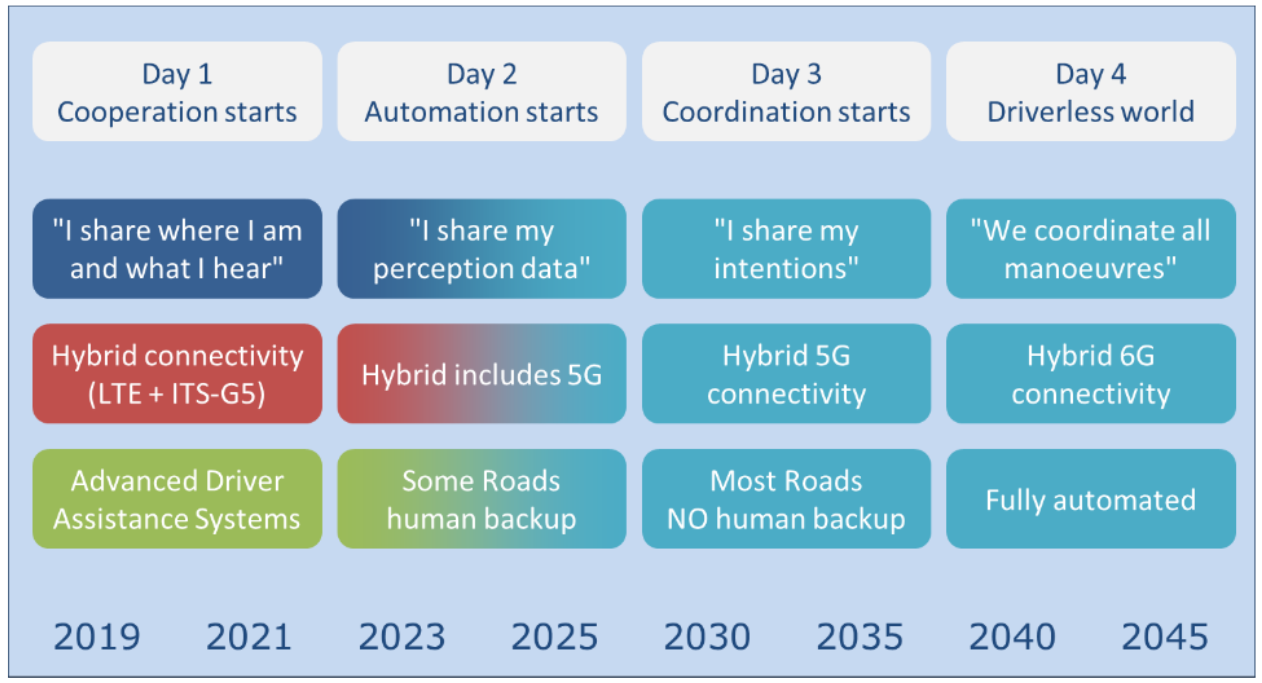
\includegraphics[width=0.8\textwidth]{Chapters/Figures/VANETs/ITS_strategy_EU.png}
   	\caption{\gls{its} strategy for the \gls{eu}~\cite{lu_pan-european_2019}}
   	\label{fig:EU_strat}
\end{figure}

% section vehicular_networks (end)

%\newpage


